\chapter{System proposal}
\label{chap:system-proposal}

Based on the information we gathered in the previous chapters, we will now propose our own \emph{application generator}. We will give a detailed description and justification of the characteristics and features that our system will have. 

At the beginning of the chapter covering Related Work (Section \ref{sec:rw:definition}), we attempted to define what a \emph{data-driven application generator} is. We admitted that this definition is rather vague and subjective but it is important because it gives as a starting point for making our own tool of this kind. We will now briefly repeat that definition.

A \emph{data-driven application generator} is a tool that takes an input data set provided by the user and produces an \emph{application} based on that data set. Defining an \emph{application} is rather difficult. For us, the main aspect is \emph{interactivity}, i.e., the generated \emph{application} will let the user interact in some way with the source data set. Moreover, a generated \emph{application} should be persistent and to an extent independent on the \emph{generator}. When the \emph{generator} is closed, the \emph{application} should not seize to exist.

\section{Proposed features}
\label{sec:proposal:features}

In Section \ref{sec:rw:features}, we presented a list features that we focused on when examining individual related tools. This list of features allowed us to compare the tools between each other in a more organized way. This list also contains the exact features that we would like our tool to have. Let us walk through that list again and explain why we think our \emph{application generator} should support these features.

\begin{itemize}
\item \emph{Linked Data support}. The majority of the examined tools supported only some kind of tabular data. That proved itself to be a very limiting factor. Each tool required the user to somehow provide the missing \emph{semantic} information (e.g. by describing the data using a \emph{schema}) and even then the tool either generated applications that looked all more or less the same (Miga Data Viewer, Citadel on the Move), or required the user to manually build the whole application (Tableau, Avelca, Exhibit). Linked Data carry way more \emph{semantic} information with them and can be \emph{understood} by the \emph{application generator}. That means that the process of generating applications can be automated (the user does not have to explain to the \emph{generator} what the input data mean) and also as the Linked Data can express way more kinds of information, way more types of applications can be generated from that data.
\item \emph{Extendability}. All applications generated for example by Miga Data Viewer looked more or less the same.  This is caused to a large extent by the characteristics of the tabular data. Linked Data, on the other hand, are way more versatile, potentially allowing way more diverse applications. However, we can hardly imagine that we could come up with a universal solution that would work for any type of data and would at the same time use up the full potential of those data. Therefore making the \emph{generator} extendable with new types of applications for different types of data is a necessity.
\item \emph{Data analysis}. A \emph{generator} that automatically analyzes the input data and makes decisions based on how it \emph{understands} the data, is definitely a more capable \emph{generator}. This is directly related to the \emph{Linked Data support}. It is the Linked Data that allow such analysis possible (we are not claiming that it is not possible to run some kind of smart analysis on tabular data, but as it would involve lots of guessing, the results might be debatable). Just to repeat what we have already said: such a smart \emph{application generator} can significantly speed up the process of application generation by making it \emph{semi-automatic} and it can support significantly more types of information with significantly more types of applications.
\item \emph{Online sharing}. Being able to \emph{share} the final generated application with others is the purpose of all these efforts. We aim to use the whole potential of the data around us and keeping our findings just to ourselves would clearly waste that potential.
\item \emph{Non-developers friendly}. Miga Data Viewer or Exhibit proved that even tools that require their users to have some programming skills, can help a lot by reducing the amount of work necessary for generating an application. Also these tools typically offered a high level of flexibility. Nevertheless, most of our potential users have zero developer skills and we would like to allow these users to generate applications using our \emph{application generator}.
\item \emph{Platform}. Tools in the form of an online platform (Avelca, Tableau, Citadel on the Move, Payola) clearly make the whole agenda around applications (creating, managing, sharing) simpler for the user. We want our tool to work as a platform as well.
\item \emph{Configuration}. We have seen two extremes among the examined tools. LinkedPipes Visualization simply produced the visualization and gave user no possibility to configure it before publishing. Tools like Tableau, Avelca or Exhibit, on the other hand, represented the other extreme. The user had to actually \emph{build} the whole application from scratch. Miga Data Viewer was somewhere in between. Most of the application was automatically generated but the user was still allowed to change certain aspects. This is the way that we would like to choose for our \emph{application generator} as well. We want to find a compromise solution that would allow the user to quickly generate new applications and yet it would still give him some space to influence how the application should look like before it gets published.
\item \emph{Level of automation}. The same argumentation that has been used for \emph{configuration} applies here as well. Based on our findings, making the \emph{application generator} \emph{semi-automatic} is the way to go. It is worth mentioning that it is the \emph{data analysis} that makes the \emph{semi-automation} possible and truly helpful. Thanks to its ability to actually understand the data, the \emph{generator} can help with the generation process, making it faster and smoother.
\end{itemize}

\section{Advantages and disadvantages of the integration into LinkedPipes Visualization}
\label{sec:system_proposal:integration}

We proposed that some kind of \emph{data analysis} should be a part of our \emph{application generator}. Automatic analysis of Linked Data, however, is a vast topic. Within the scope of this thesis, we would be probably able to come up only with a very basic solution consisting of simple rules such as  \textit{"This entity is an address or GPS coordinates, let us display it on a map."} or \textit{"These are some statistical data, let us visualize it using a graph"}. We can say that Miga Data Viewer works in similar way.

We believe that it is not always necessary to reinvent what has been already invented and that we would rather give ourselves a head start by re-using an existing solution. For various reasons, we decided to integrate our \emph{application generator} into LinkedPipes Visualization. Let us now walk through those reasons.

\begin{enumerate}
\item Through LinkedPipes Visualization we get a strong analytical framework that we can immediately use. We will utilize the \emph{discovery} algorithm which will automatically tell use how the input data can be visualized, i.e., what kinds of applications can be generated.
\item We will greatly benefit from the LinkedPipes Visualization implementation of LVDM. Firstly, it will make our generator easily extendable to support new types of data through new LDVM components. Secondly, any LDVM component following the format defined by this implementation will automatically work in our generator as well (with the limitations explained in Section \ref{sec:linkedpipes:component_registration}).
\item On a programming level, LinkedPipes Visualization already contains lots of ready-to-use solutions for working with RDF data (querying Virtuoso triplestore, converting RDF to JSON etc.). It also offers a programmatical API providing a direct access to the \emph{discovery} algorithm (launching, accessing results etc).
\item Finally, we admit that what played an important role in our decision process was the fact that we had direct access to the authors of LinkedPipes Visualization. That significantly sped up our work.

\end{enumerate}
If we decided not to use LinkedPipes Visualization as the base for our \emph{generator}, we would have to either adopt another solution or create the \emph{generator} from scratch. To our best knowledge, there is no project that would provide an automatic analysis of Linked Data similar to what LinkedPipes Visualization offers. LDVM \cite{ldvm} and its implementation \cite{ldvm_use_cases} in LinkedPipes Visualization were created specifically because of the lack of such a tool. As of creating the \emph{generator} from scratch, we already suggested how that would look like in the introduction paragraph of this section. We would probably come up with a similar solution, yet immensely simpler and less powerful. The third option would be to get rid of the \emph{data analysis} and make the \emph{application generator} fully \emph{manual}. As we argued in Section \ref{sec:proposal:features}, we prefer our \emph{generator} to be rather \emph{semi-automatic}.

This decision has also disadvantages. The original guidelines for this thesis suggest that the user should be able to combine together different views for different types of data. Such views should be possible to display in a selected predefined layout before publishing the app. We have seen this approach for example in Tableau. However, LinkedPipes Visualization visualizers use a completely different approach. They are typically domain specific. Each visualizer focuses on a single type of data, for example map data, and then offers a rich (but static) user interface which is specifically designed to work with this particular type of data (for example, it displays controls allowing the user to filter the visualized data). This is a direct consequence of the underlying LDVM pipeline \emph{discovery} algorithm.

Unfortunately, if we are to build on top LinkedPipes Visualization and use its full potential, our applications (which will directly correspond to the \emph{visualizers}) cannot look and work much differently. Nevertheless, these are two vastly different approaches that both are viable and both have their advantages and disadvantages. By adopting the approach of domain-specific applications, we will reduce the application configurability and it will not be possible to generate dashboard-like applications known from Tableau. On the other hand, our domain-specific applications will offer richer user interfaces allowing more advanced work with the visualized data. Moreover, we are convinced that this approach has more use-case scenarios. It is possible that the user decides to use as an input a large data set, like DBPedia~\cite{dbpedia}, or a combination of many smaller data sets, that would contain lots of different data, potentially resulting in many discovered \emph{pipelines} and therefore many different visualizations. Those would make sense to be organized in a dashboard-like application. Such a scenario, however, is not very probable.

\section{Contribution}
\label{sec:system_proposal:contribution}

We already classified LinkedPipes Visualization as an \emph{application generator} when we were comparing related tools. The reader might ask how exactly is our \emph{application generator} going to be better. 

\subsection{Configuration phase}

\begin{figure}
	\centering
	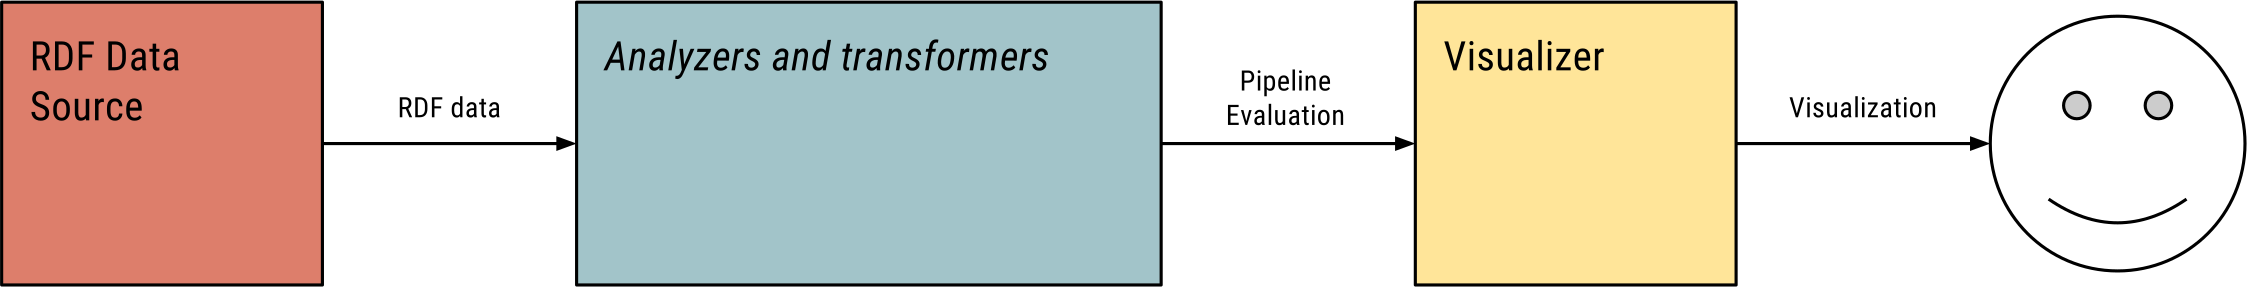
\includegraphics[width=135mm]{img/04_pipeline_scheme_lpv.png}
	\caption{Pipeline schema in LinkedPipes Visualization. The \emph{pipeline evaluation} is directly passed to the \emph{visualizer} which produces the final visualization. The process is fully automatic with zero input from the user.} 
	\label{fig:pipeline-scheme-lpv}
\end{figure}

In LinkedPipes Visualization, when the user selects and executes a \emph{pipeline}, he is redirected to the corresponding \emph{visualizer} user interface. That generates the actual \emph{visualization} from the \emph{pipeline evaluation} (Figure~\ref{fig:pipeline-scheme-lpv}). In the context of LinkedPipes Visualization, that is the generated application. In our \emph{application generator}, we will introduce a configuration phase that will precede the publication. Each \emph{visualizer} will consist of two user interfaces: a \emph{configurator} interface and an \emph{application} interface. 

\begin{figure}
	\centering
	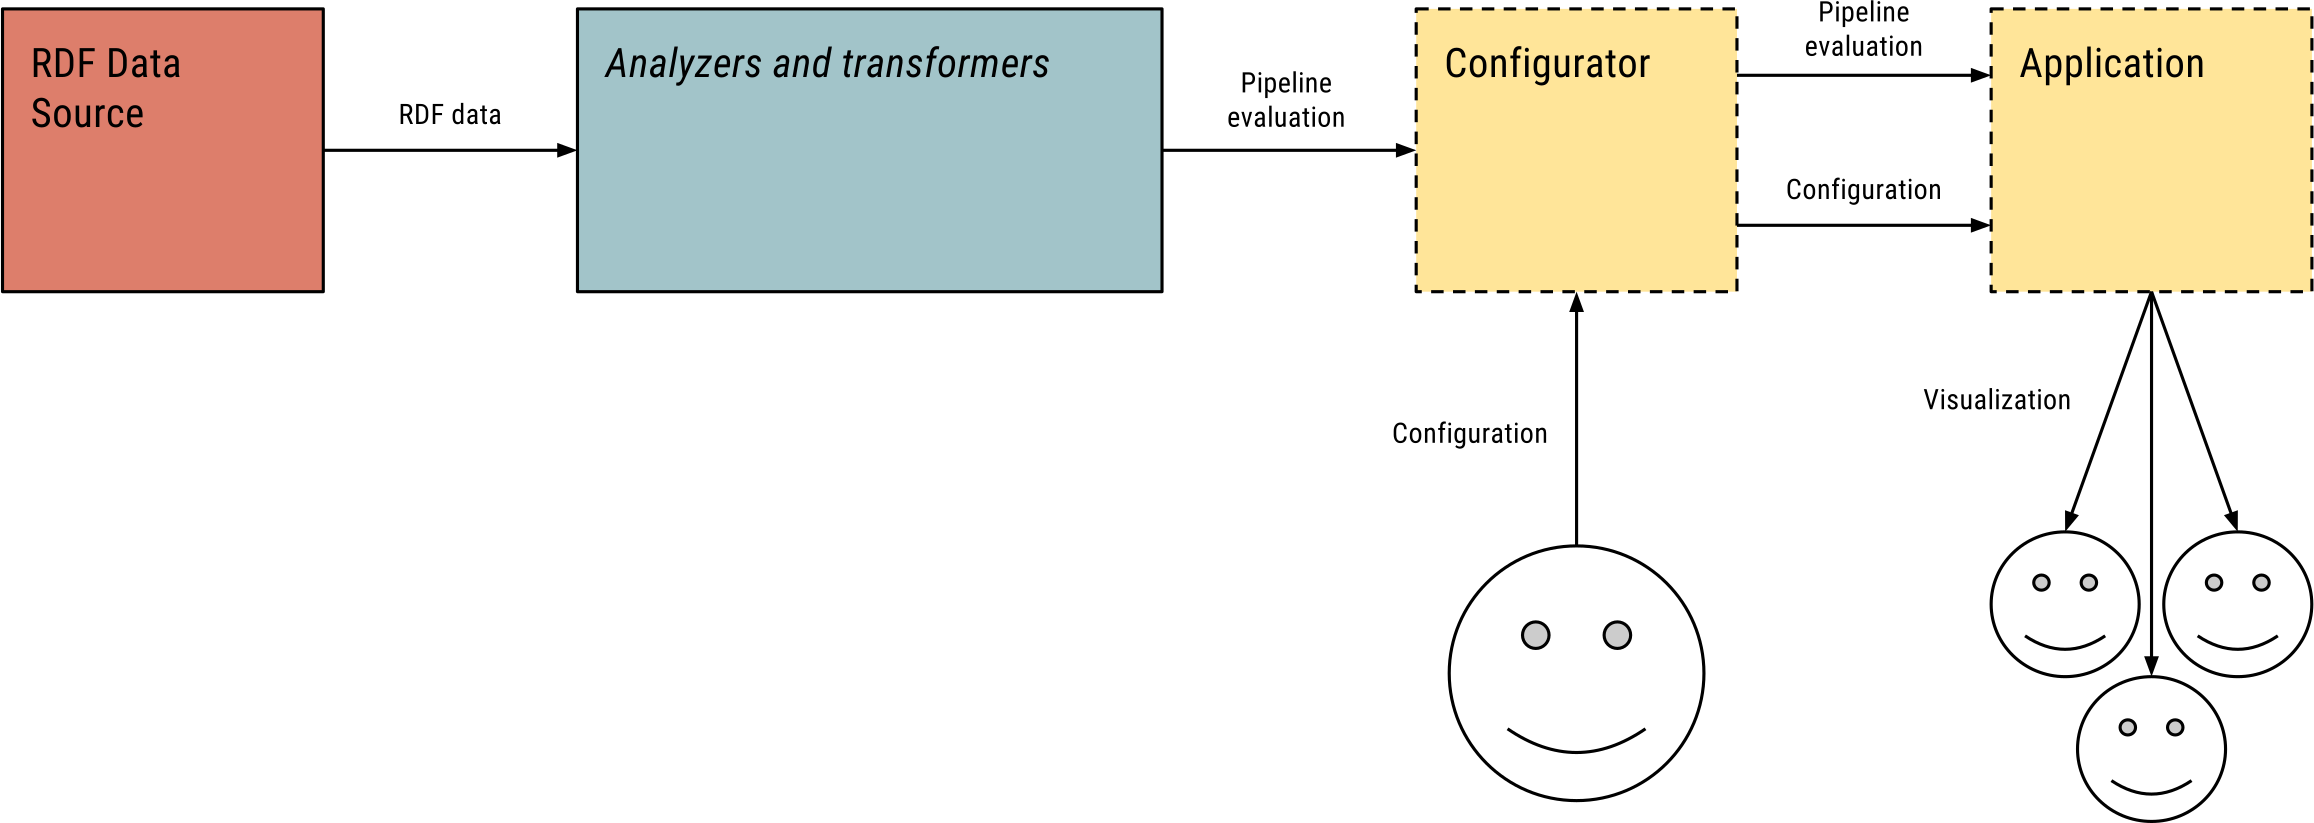
\includegraphics[width=140mm]{img/04_pipeline_scheme_appgen.png}
	\caption{Pipeline schema in the \emph{application generator}. The user creating the application can provide further configuration which will affect how the final application presented to the audience will look like. Compared to LinkedPipes Visualization, the \emph{application generator} introduces the \emph{configurator} and \emph{application} user interfaces (marked with dashed borders).} 
	\label{fig:pipeline-scheme-appgen}
\end{figure}

The \emph{configurator} interface will let the user to shape the application before publishing (Figure~\ref{fig:pipeline-scheme-appgen}). The configuration possibilities will differ depending on the \emph{visualizer}, but typically the user will be allowed to filter the data (select a subset) and tune the level of interactivity for the audience.

Let us say that we are working with the Google Maps Visualizer and our data set contains geospatial points divided into a large number of categories. 

\begin{itemize}
\item The user could create a \textbf{completely static} visualization by selecting one (or more) of the categories to be visualized and fixing them (i.e., the audience will not be able to change them). This will result in a static map with fixed points (very convenient for embedding into external web pages).
\item The user could create a \textbf{partially dynamic} visualization. As the number of categories might be too large, the user could select only a couple of them but this time he would allow the audience to arbitrarily choose which categories they want to visualize.
\item The user could create a \textbf{fully dynamic} visualization by leaving all categories enabled, giving the audience full control over the visualization. This corresponds to what LinkedPipes Visualization would produce.
\end{itemize}

This will greatly increase the re-usability of data sets and \emph{visualizers}. A single data source with a single \emph{visualizer} will work as a potential source for many applications, each serving a different purpose (and a different target audience).

The \emph{application} interface is what the end-user (the audience) is going to see. When describing how a \emph{visualizer} works in LinkedPipes Visualization (Section \ref{sec:linkedpipes:visualizers}), we stated that a \emph{visualizer} is a function that takes the \emph{pipeline evaluation} as an argument and returns the actual \emph{visualization}. In our \emph{application generator}, the \emph{application} interface will be a function with two arguments: the \emph{pipeline evaluation} and the configuration created in the \emph{configurator} (Figure~\ref{fig:pipeline-scheme-appgen}).

By introducing the configuration phase, we created another level of abstraction. The process of generating a new application (which includes the configuration phase now) requires no programming skills. It is very \emph{non-developer friendly}. But it does require certain understanding of the data and making sense out of the data (e.g. creating a meaningful graph) might require quite a lot of effort. In LinkedPipes Visualization, any user has to put in this effort when using the generated \emph{visualization}. In our \emph{application generator}, only the user generating the application will have to make this sacrifice during the configuration phase, but the end user (the audience) will get only the final refined application.

Another problem that the configuration phase addresses is the potential overall poor data quality. For example according to~\cite{dbpedia_quality}, $11.93\%$ of evaluated triples from DBpedia~\cite{dbpedia} suffer from some quality issues.  Clearly, the configuration phase presents an opportunity to deal with these issues before the visualization reaches the audience. This may take a form of creating a partially dynamic visualization (as explained above) that would simply hide the corrupted data from the user. To give the reader a more specific example, a typical problem that the user might face while creating an application could be missing or incorrect labels of visualized RDF resources. The configurator will allow to provide a custom label for any such visualized RDF resource.
\begin{figure}
	\centering
	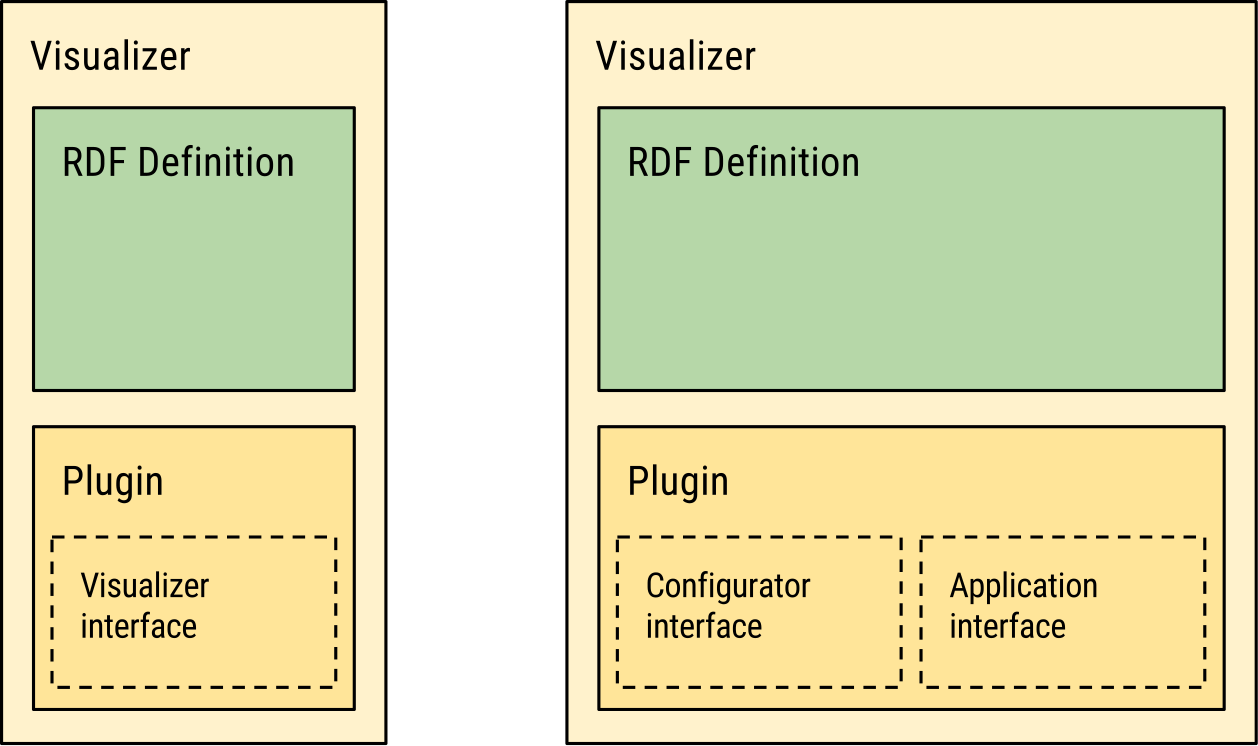
\includegraphics[width=100mm]{img/04_visualizer_comparision_scheme.png}
	\caption{Comparison between a \emph{visualizer} structure in LinkedPipes Visualization (on the left) and in our \emph{application generator} (on the right). } 
	\label{fig:visualizer-comparison-scheme}
\end{figure}

We should also eliminate any confusion in the terminology that might have arisen in this section. A \emph{visualizer} is the last LDVM component in a \emph{pipeline}. It consists of the RDF definition and of the actual implementation in the code (the \emph{plugin}). The RDF definition is always the same, but the  \emph{plugin} will differ for LinkedPipes Visualization and of our \emph{application generator}. In the latter case, a \emph{visualizer} will consist of the aforementioned \emph{configurator} interface and \emph{application} interface. See Figure \ref{fig:visualizer-comparison-scheme}. In a sense, it will work as an \emph{application template} for generating new applications. Nevertheless, we will stick to the term \emph{visualizer} in the rest of this text.

\subsection{Platform}

LinkedPipes Visualization is a technical successor of Payola but it dropped most of Payola's platform features along the way. We will give them back, at least to the extent that makes sense for our cause. As our applications will be configurable, we will build necessary infrastructure around application management. That includes also support for registering and authenticating users.

Moreover, one of the Payola's important features was sharing and re-using of the \emph{plugins}. This also works in LinkedPipes Visualization. The \emph{discovery} algorithm is using all available LDVM components. But when a user wants to specifically run the \emph{discovery} algorithm on a selected \emph{data source} that already exists in the system, it is not possible. It is only possible to tell the \emph{discovery} algorithm that it should try to combine the new \emph{data source} with the existing ones. That process is, however, also fully automatic, i.e., it is not possible to specify which ones the \emph{discovery} algorithm should use. It will always use all of them.

We will make a simple database of available data sets part of our \emph{application generator}. The idea is that some users will be responsible for producing interesting data sets and the platform will allow them to share the data sets with other users who will use them to generate applications. Also a simple catalog of published applications will be part of the platform.

In general, the whole user interface of LinkedPipes Visualization is rather bare and simplistic as its point is merely to show the capabilities of the underlying LDVM \emph{discovery} algorithm. Our aim, on the other hand, will be to create a more refined and polished product.

\subsection{Framework}

In Section \ref{sec:linkedpipes:component_registration} we described how new LDVM components  can be integrated into the code of LinkedPipes Visualization. As this tool defines a clear way how it can be extended, we can say it also fits into the role of a framework for implementing new types of Linked Data visualizations. Also when we were talking about the advantages and disadvantages of integrating our generator into LinkedPipes Visualization (Section \ref{sec:system_proposal:integration}), we mentioned that on a programming level, we will be able to utilize various available APIs for working with RDF data. Unfortunately, LinkedPipes Visualization offers no such help for development of the \emph{visualizer} user interface.

Our \emph{visualizers} are different. In front of all, they are more complicated because they consist of two different user interfaces, the \emph{configurator} and \emph{application}. The framework will have to define a clear way how to seamlessly integrate both of these interfaces into the generator.

We will define a recommended structure for the \emph{configurators} which will speed up their implementation. Thanks to this unified structure, it will be possible to leverage ready-to-use solutions for some common tasks, e.g. saving and loading the application configuration, universal support for multiple languages and adding/editing labels of RDF data. On the server side, we will provide a universal persistent request cache to increase the performance of published applications. None of these features are currently available in LinkedPipes Visualization.

Naturally, thanks to the framework, the user will not have to deal with any of the platform related tasks (e.g. authentication or authorization) and the platform features will be provided to him via explicit API (e.g. access to currently authenticated user).

\section{Visualizers}

To showcase the capabilities of our \emph{platform} and \emph{framework}, we will implement and present to the user two \emph{visualizers}. The first one will be a brand new D3.js Chord Visualizer based, as the name suggest, on the D3.js chord layout, capable of visualizing directed weighted graphs. The other one will be based on the existing LinkedPipes Visualization map visualizer. The RDF definition will remain the same, we will just re-implement the \emph{visualizer} for our \emph{application generator}.

\section{Mockups}

In this subsection we will briefly present to the reader our idea of  the \emph{application generator} user interface. The core parts are the process of generating a new application and configuring an existing application. Let us start with generating an application.

In the first step (Figure \ref{fig:mockups_select_datasources}), the user has to select the RDF data sources. Unlike LinkedPipes Visualization, our \emph{application generator} will offer a user-friendly browser of available data sources (the \textbf{Browse} button on Figure \ref{fig:mockups_select_datasources}) which means that the user will not be forced to deal with notions like SPARQL endpoint, named graph or TTL file. On the other hand, the more advanced users will be allowed to add their own RDF data sources (the \textbf{Add new} button).
\begin{figure}
	\centering
	\includegraphics[width=140mm]{img/04_mockups_select_datasources.png}
	\caption{Step 1: Selecting data sources. The user is allowed to select an arbitrary number of data sources, either from the already available ones using the browser, or by providing new ones.} 
	\label{fig:mockups_select_datasources}
\end{figure}
\begin{figure}
	\centering
	\includegraphics[width=140mm]{img/04_mockups_discovery.png}
	\caption{Step 2: Running \emph{discovery} algorithm. The screen shows current progress including already discovered \emph{pipelines}.} 
	\label{fig:mockups_discovery}
\end{figure}

Once the user is happy with his selection, he hits the \textbf{Run Discovery} button and is redirected to the next screen (Figure \ref{fig:mockups_discovery}) where he can watch the progress of the \emph{discovery} algorithm. As new \emph{pipelines} are discovered, they are shown on the screen, grouped by their LDVM \emph{visualizer} component. That means that unlike in LinkedPipes Visualization, the user can easily see what kinds of visualizations (or applications) are possible from selected data sources. The user first decides for a \emph{visualizer} and then clicks the appropriate \textbf{Show pipelines} button (Figure~\ref{fig:mockups_discovery}) which will open a list of discovered \emph{pipelines} for the chosen \emph{visualizer}.

\begin{figure}
	\centering
	\includegraphics[width=140mm]{img/04_mockups_configurator.png}
	\caption{Sample \emph{configurator interface}. The upper part is for all \emph{visualizers} identical, covering common functionality, the lower part is custom. In this case, the application visualizes entities on a map.} 
	\label{fig:mockups_configurator}
\end{figure}

Now the user selects one of the discovered \emph{pipelines} and executes it which will process the data from the data sources and transforms them (according to the \emph{pipeline} structure). This might take a while. Once the \emph{pipeline evaluation} finishes, the user can create a new application from it. Unfortunately, we are not able to help the user in any way with choosing a \emph{pipeline}. If there are multiple \emph{pipelines} available for a single \emph{visualizer}, the user might have to try all of them to see which gives him the best results.

When an application is created, the user is taken to the \emph{configurator} interface (Figure \ref{fig:mockups_configurator}) where he can modify the application before it gets eventually published.

\section{Architecture analysis}
\label{sec:system-proposal:architecture-analysis}

We decided that we would build our \emph{application generator} on top of LinkedPipes Visualization (Section \ref{sec:system_proposal:integration}). We already described the architecture of this tool (Section \ref{sec:linkedpipes:architecture} and especially Figure \ref{fig:linked-pipes-visualization-architecture}). We will now describe the way the \emph{application generator} is integrated into LinkedPipes Visualization, including the overall software architecture.

\subsection{Integration into LinkedPipes Visualization}
\label{sec:system-proposal:architecture-analysis:integration}

There were two basic ways how we could approach the integration:

\begin{enumerate}
\item Make the \emph{application generator} a part of LinkedPipes Visualization, i.e., directly integrate the \emph{application generator} into the codebase.
\item Develop the \emph{application generator} as a separate application and use an instance of LinkedPipes Visualization as a service providing required functionality via a remote (HTTP) API.
\end{enumerate}

As of the second approach, the architecture of LinkedPipes Visualization (Figure \ref{fig:linked-pipes-visualization-architecture}) would be well suited for it. The backend of LinkedPipes Visualization exposes its functionality (including the LDVM implementation) to the frontend via a public HTTP API. We could immediately use that API in our \emph{application generator}. In general, this would be the cleanest approach from the software architectonic perspective.

Unfortunately, it turned out that if we used LinkedPipes Visualization as a separate service, we could not avoid changes in the codebase of LinkedPipes Visualization. Consider, for example, how a \emph{visualizer} works (see Subsection \ref{sec:linkedpipes:visualizers} for the complete workflow). An important part of a \emph{visualizer's} job is to take the \emph{pipeline} output (which is in RDF) and convert it into a format suitable for the visualization itself (typically JSON). This conversion routine would clearly differ for each \emph{visualizer} as each \emph{visualizer} would be dealing with different kind of data. In LinkedPipes Visualization, this happens on the backend, i.e., each \emph{visualizer} exposes its own public API providing the data extracted from RDF in JSON. The consequence for us is pretty clear: if we wanted to extend our \emph{application generator} to support another type of RDF data, i.e., add another \emph{visualizer}, we would need to extend LinkedPipes Visualization as well. 

A possible solution to this problem would be to alter the public API of LinkedPipes Visualization to return the original RDF data instead and move this custom \emph{visualizer} functionality (we referred to it as to a \emph{plugin}, see Subsection \ref{sec:linkedpipes:ldvm-implementation:component-representation}) to the \emph{application generator}. Working with RDF, however, is a bit complicated and the codebase of LinkedPipes Visualization already contains several ready-to-use solutions that, among other things, significantly speed up the process of implementing support of new types of RDF data (new vocabularies). We could surely use those solutions in our \emph{application generator} but to make them available there, we would need to transfer them somehow (i.e., duplicate) or come up with a way how to share them between the \emph{application generator} and LinkedPipes Visualization.

\begin{figure}
	\centering
	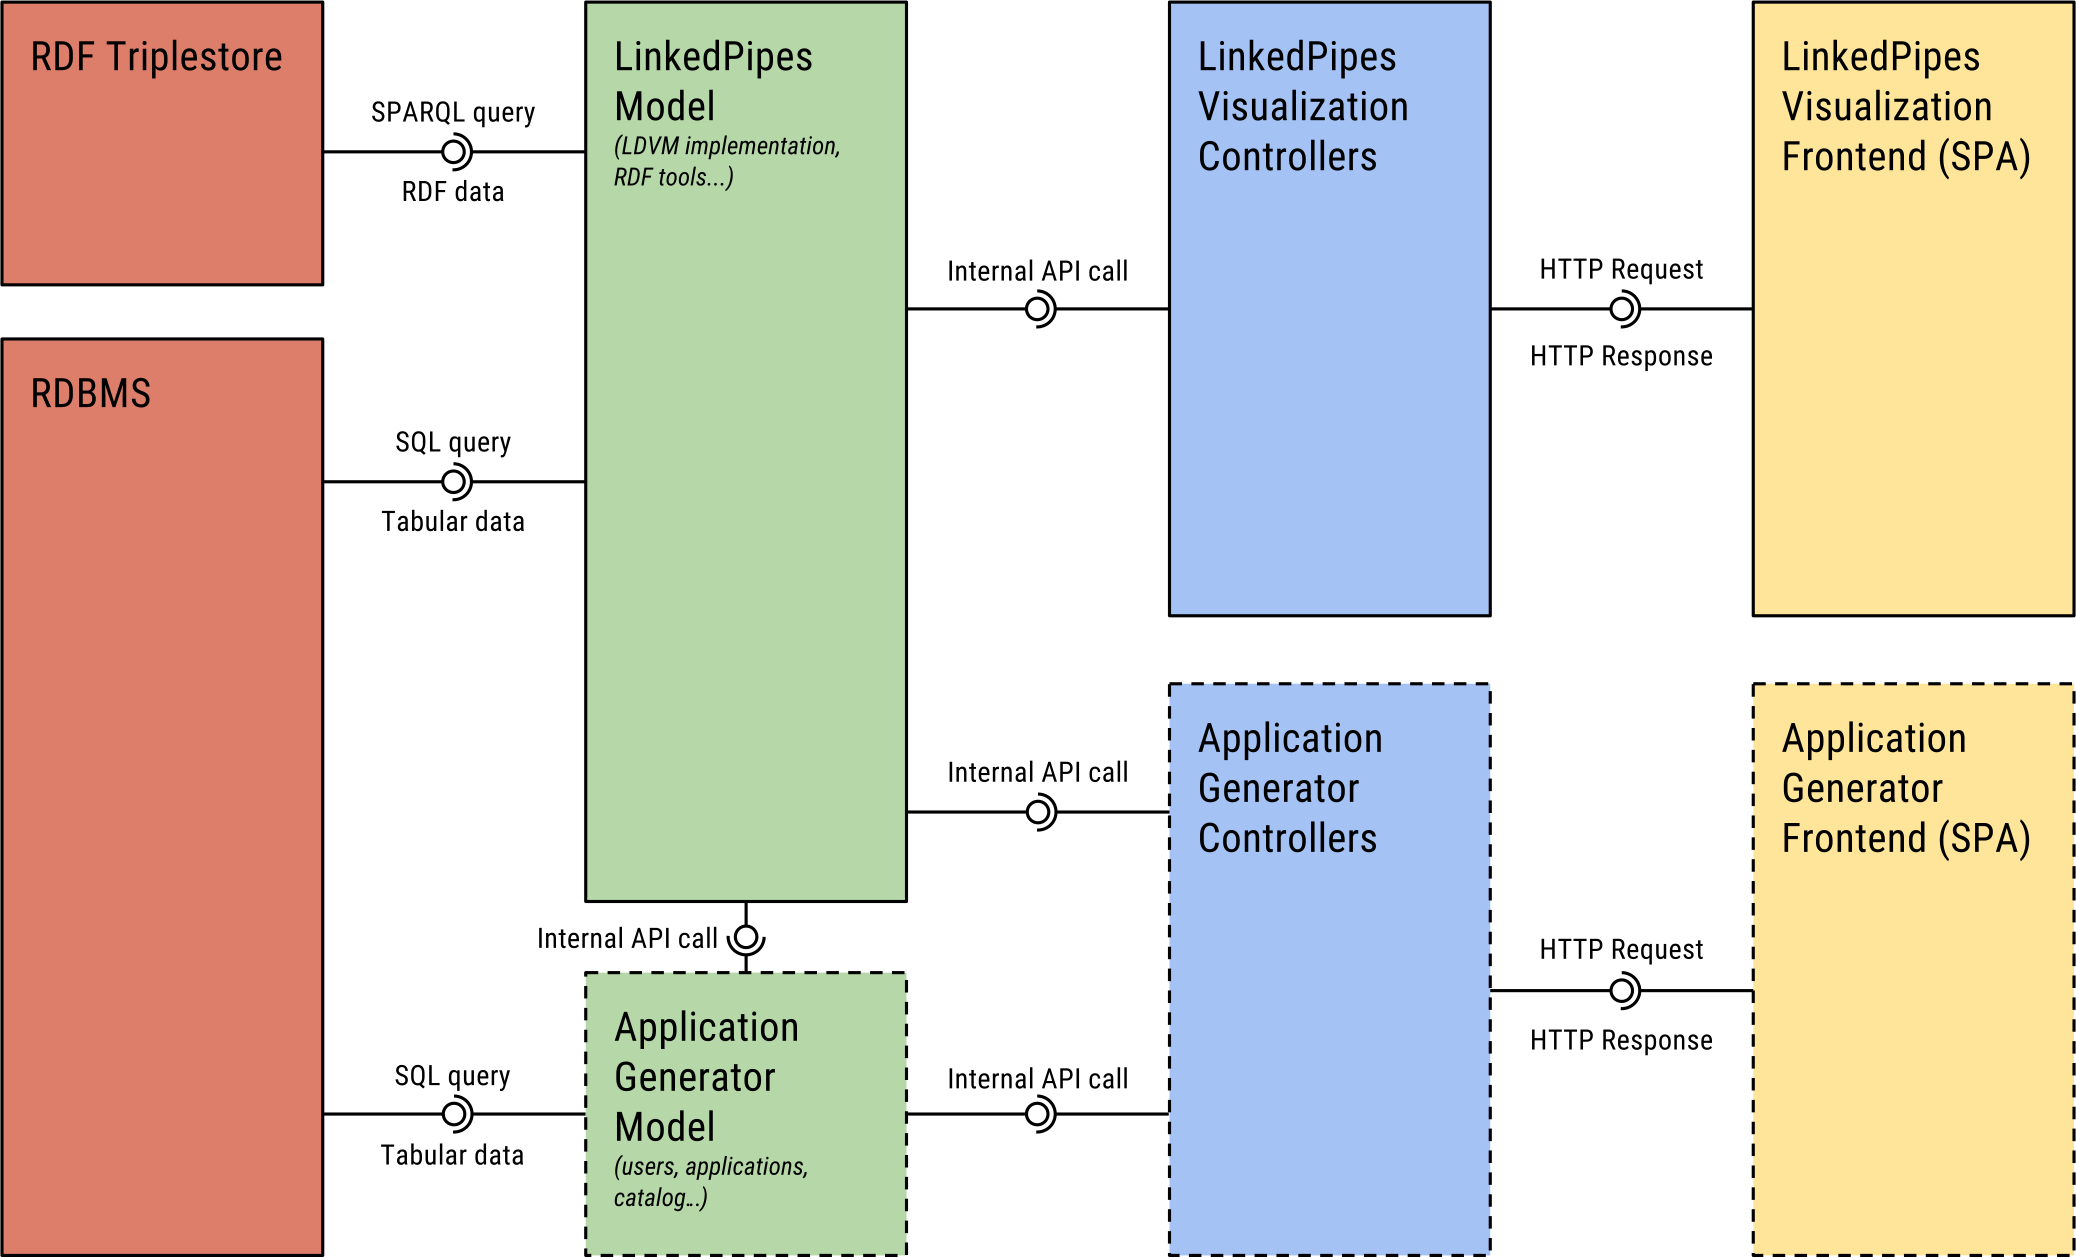
\includegraphics[width=140mm]{img/04_application_generator_architecture.png}
	\caption{Architecture of the \emph{application generator}. Blocks with solid borders are part of the original LinkedPipes Visualization, blocks with dashed borders are newly implemented parts of the \emph{application generator}. The backend follows the standard MVC architecture.} 
	\label{fig:proposed-application-generator-architecture}
\end{figure}

Coming to this realization, we decided to take the path of least resistance and integrate our \emph{application generator} directly into the LinkedPipes Visualization codebase, just as the fist approach suggests. As the result, we could immediately start utilizing the existing patterns and tools for working with RDF. 
very
Nevertheless, even though both tools live in the same code base, we made sure to keep them as separated as possible. So if we decided in the future to separate both tools or for example replace the underlying LDVM implementation, it should be rather straightforward. How this is achieved can be seen on Figure \ref{fig:proposed-application-generator-architecture}. We will walk through the individual layers of integration in the following subsections.

An important consequence of this unification is that the LDVM implementation instance is shared among the \emph{application generator} and LinkedPipes Visualization. That means that they both use the same set of registered LDVM \emph{components}. We benefit from this as well to an extent as we can utilize existing implemented user interfaces handling some of the LDVM related tasks (e.g. new LDVM \emph{components} are registered to the \emph{generator} through the LinkedPipes Visualization user interface).

\subsection{Frontend integration}
\label{sec:system-proposal:architecture-analysis:frontend-integration}

In LinkedPipes Visualization, the frontend is an SPA living in the client web browser. Its responsibility is to render the user interface which communicates with the backend using the public remote API via HTTP. The frontend part does involve some more complex logic, e.g. necessary for rendering the visualizations themselves, but in general all core business logic (anything related to RDF, the \emph{discovery}, any data transformation or filtering) is almost exclusively dealt with in the backend and the frontend merely serves as the way to communicate with the user. The \emph{application generator} frontend follows this approach as well.

There was an option to re-use the original frontend and just extend it with the functionality that we needed. It already contained some work that we could at first glance use (for example frontend parts of existing \emph{visualizer} plugins, i.e., the actual visualizations). Unfortunately, couple of problems prevented us from doing so. 

\begin{enumerate}
\item The frontend was created just to showcase the capabilities of the underlying LVDM implementation. For this reason, the overall code quality was not  a number one priority. The code was not structured well enough so that we could start extending it. In general, it would take us lots of time to get familiar with it. 
\item The code was not written with certain features (like for example user support or the aforementioned general extendability) in mind.
\item Our \emph{visualizers} (with the separated \emph{configurator} and \emph{application} interfaces) work very differently compared to the \emph{visualizers} of LinkedPipes Visualization.

\end{enumerate}
Having these three reasons in mind, we came to the conclusion that we would have to rewrite a major portion of the original code anyway and therefore we decided to start from the scratch. As a result, there are two existing user interfaces that live within the same application next to each other, available from two different starting URLs.

\subsection{Frontend architecture}
\label{sec:system-proposal:architecture-analysis:frontend-architecture}

The frontend itself can be viewed as a standalone application that has its own inner architecture. It is responsible for rendering the user interface which involves many not so simple tasks, including transitions between individual screen, processing user input, processing backend responses (including the the failed ones) and of course visualizations themselves. The architecture is also important because it defines the way the frontend can be extended with new \emph{visualizers}. 
\begin{figure}
	\centering
	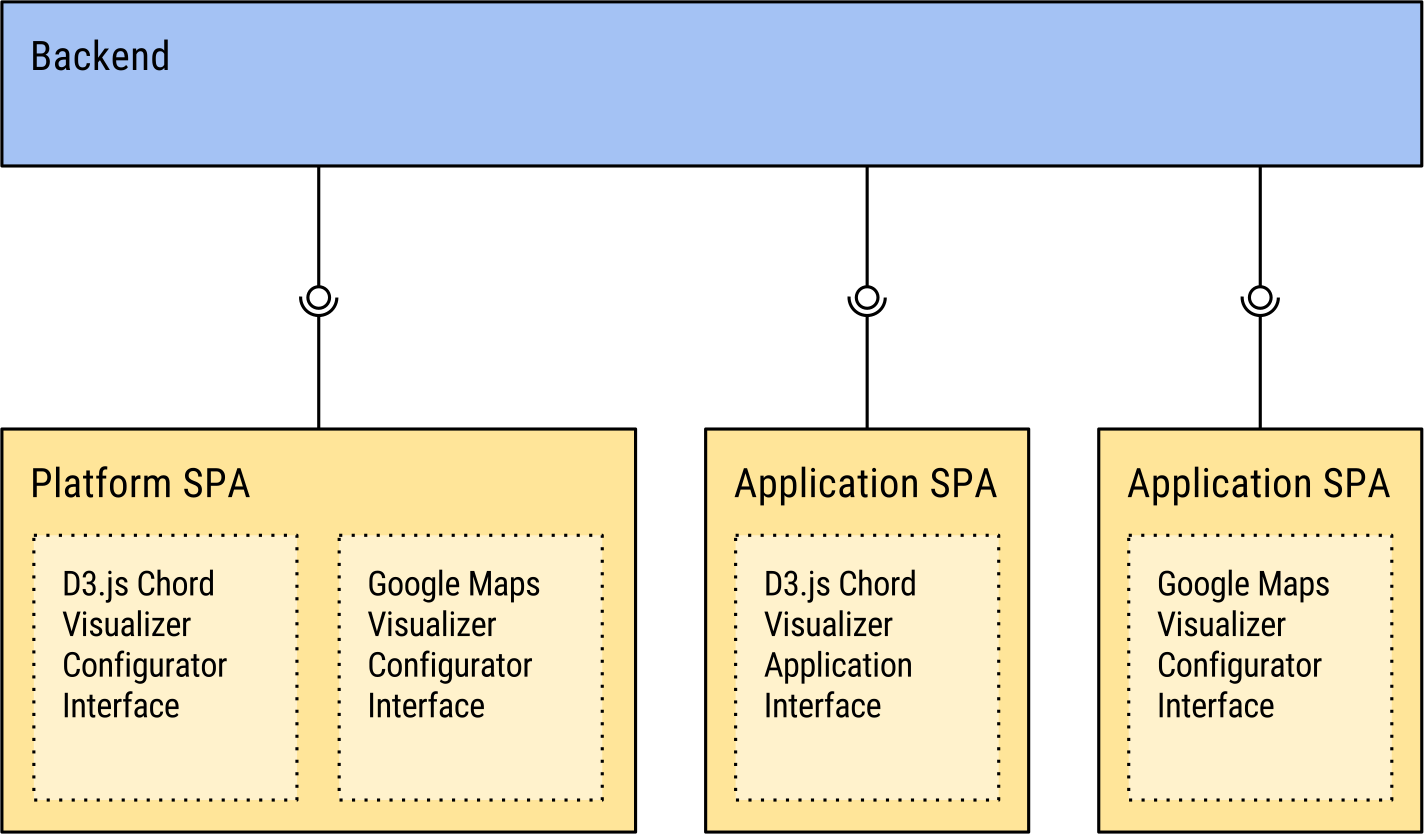
\includegraphics[width=140mm]{img/04_frontend_base_structure_spas.png}
	\caption{The \emph{application generator} frontend consists of several separated Single-page applications.} 
	\label{fig:frontend-base-structure-spas}
\end{figure}

The frontend actually consists of several standalone Single-page applications, as Figure \ref{fig:frontend-base-structure-spas} suggests. There is one big \emph{platform} SPA, which contains \emph{configurator interfaces} for all \emph{visualizers}, and then for each \emph{visualizer} there is a small dedicated SPA, which contains only the \emph{application interface} for that particular \emph{visualizer}. The \emph{platform} SPA covers the overall generator agenda which includes most importantly generating and configuring applications. Each \emph{visualizer} SPA, on the other hand, is responsible only for rendering published application of that particular type. 

When a published application is accessed, depending on the \emph{visualizer}, the appropriate SPA is loaded. On the other hand, the \emph{platform} SPA needs to deal with this problem dynamically, using an internal mechanism that loads the appropriate \emph{configurator interface} on demand. This mechanism will be described later in this subsection.
\begin{figure}
	\centering
	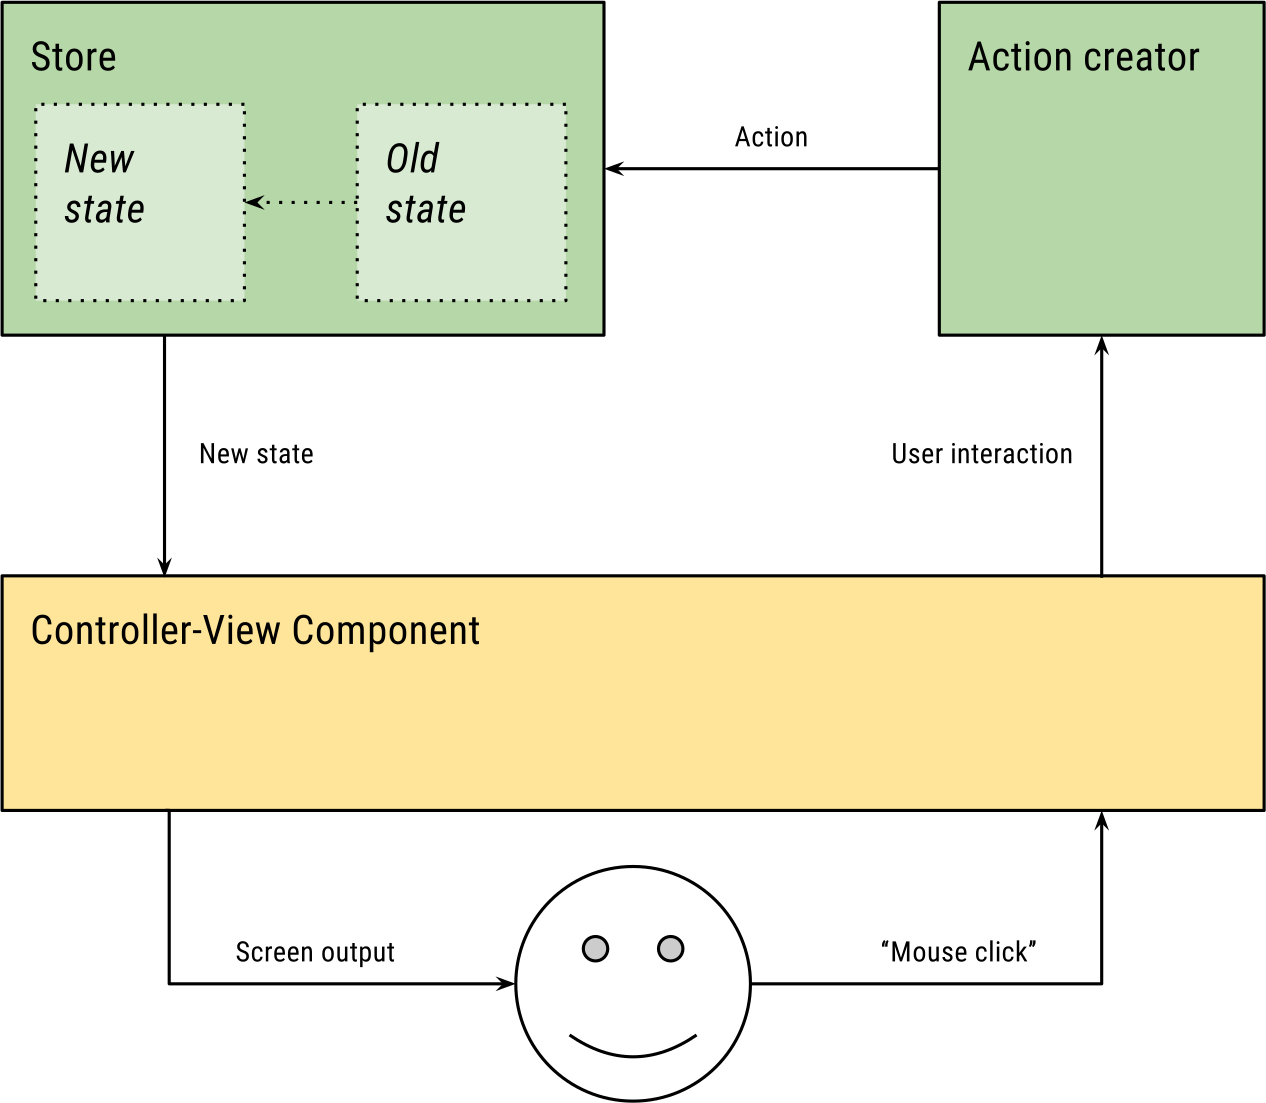
\includegraphics[width=120mm]{img/04_frontend_flux_redux.png}
	\caption{Unidirectional data flow inside an application following the Flux~\cite{flux} pattern.} 
	\label{fig:frontend-flux-redux}
\end{figure}

The inner frontend architecture follows the Flux~\cite{flux} pattern, or specifically the Redux~\cite{redux} mutation of Flux. The core idea is a unidirectional data flow, as shown on Figure \ref{fig:frontend-flux-redux}. Let us take an example of how this pattern deals with user interactions. Let us say that the user clicks a button to increase a counter's value. This is what would happen:

\begin{enumerate}
\item The user clicks the button
\item The \emph{controller-view}~\footnote{\url{https://facebook.github.io/flux/docs/overview.html}} layer intercepts that interaction and dispatches an appropriate \emph{action} to the \emph{store}.
\item The \emph{store} updates the \emph{state} using the \emph{action} and notifies the \emph{controller-view} layer of the change.
\item The \emph{controller-view} updates itself using the new \emph{state} which results in a change on the screen.
\end{enumerate}

The \emph{state} is a single hierarchically structured object that holds the complete state of the user interface, i.e., what the user sees on the screen is a function of the \emph{state}. The \emph{controller-view} layer both defines how the user interface, given the \emph{state}, should look like and how it should respond to user input. An \emph{action} represents an event that occurs in the system. It is a structured object which is identified by a unique name and can carry a payload. To create \emph{actions} we usually use factories called \emph{action creators}. The \emph{store} holds the \emph{state}, it updates it with incoming \emph{actions} and notifies the \emph{controller-view} layer of changes.

It is important that the only way the \emph{state} (and consequently the user interface) is updated, is through \emph{actions}. That means that given an initial \emph{state} and a sequence of \emph{actions}, we always reach the same \emph{state}. This aspect greatly improves the predictability of the frontend application. 
\begin{figure}
	\centering
	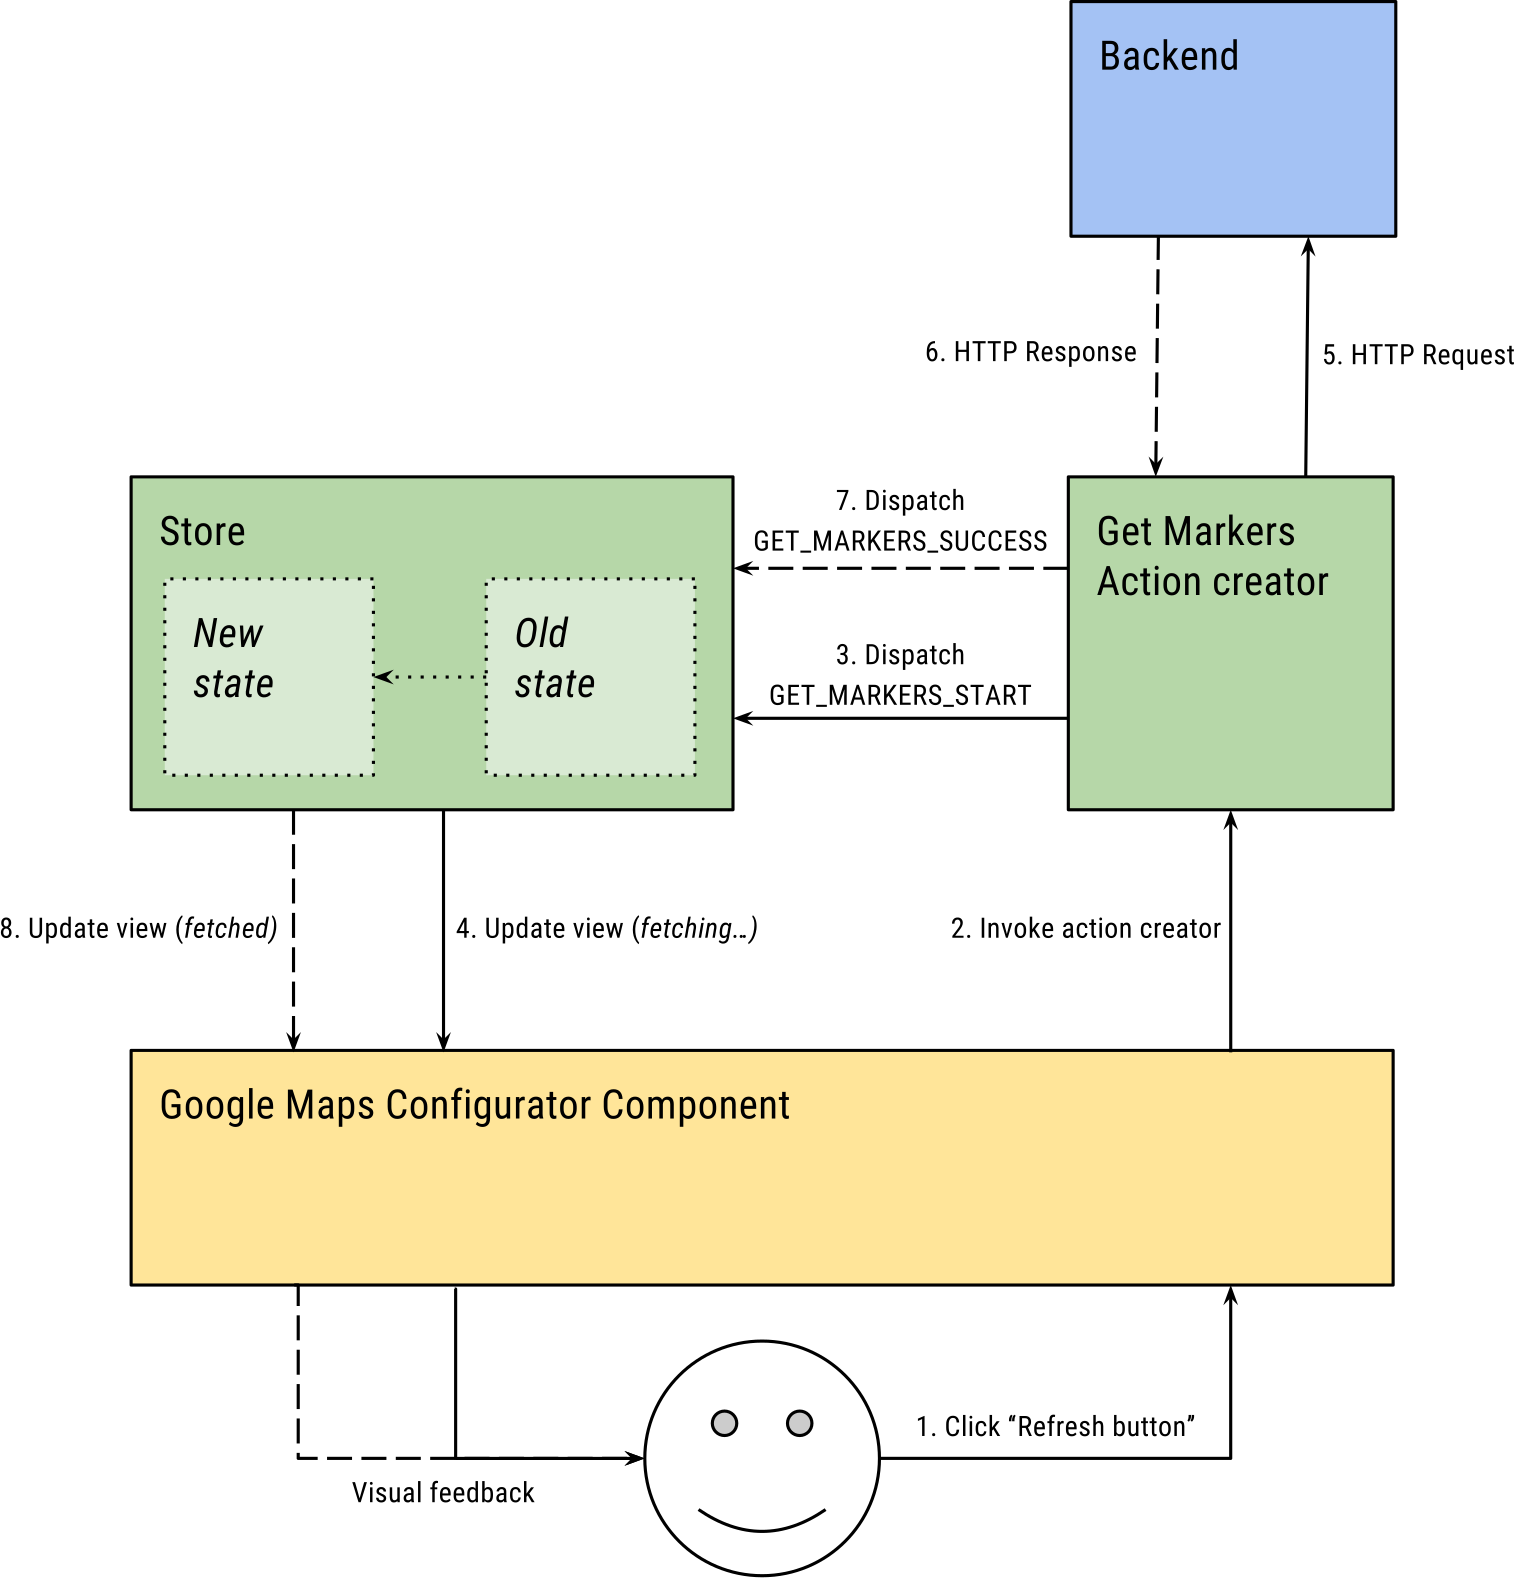
\includegraphics[width=140mm]{img/04_frontend_making_http_request.png}
	\caption{Making an HTTP request to the backend. The arrows with solid lines represent the first phase (the request is made), the arrows with dashed lines represent the second phase (the response is received).} 
	\label{fig:frontend-making-http-request}
\end{figure}

As the initial example was very simple, let us take a more complex one, which involves communication with the backend. In this example, the user clicks the \textbf{Refresh} button (see mockup Figure~\ref{fig:mockups_configurator}) to load updated markers from the server to be shown on a Google Map. The whole process is visualized on Figure~\ref{fig:frontend-making-http-request}. It consists of the following steps:

\begin{enumerate}
\item The user clicks the \textbf{Refresh} button.
\item The \emph{controller-view} layer (represented by a \texttt{Google Maps Configurator Component} at this moment) intercepts the click and invokes \texttt{Get Markers Action Creator}.
\item The \emph{action creator} firstly dispatches the \texttt{GET\_MARKERS\_START}  action.
\item The \emph{store} updates the \emph{state} accordingly (let us say that an appropriate boolean variable \texttt{loading} is flipped to \texttt{true}) and informs the \emph{controller-view} layer of this change which results in a user interface update and consequently visual feedback on the screen (e.g. the user will see an animated loading indicator).
\item The \emph{action creator} makes the actual HTTP request to the backend to get the markers and waits for the response.
\item The backend responds with the markers.
\item The \emph{action creator} dispatches the \texttt{GET\_MARKERS\_SUCCESS} action with the received markers as the action payload.
\item The \emph{store} updates the \emph{state} accordingly (the aforementioned variable is flipped back to \texttt{false} and the markers are stored in the state). The \emph{controller-view} layer is notified of another changes and updates itself according to the new \emph{state} (e.g. the loading bar is hidden and the markers are shown on the map).
\end{enumerate}
\begin{figure}
	\centering
	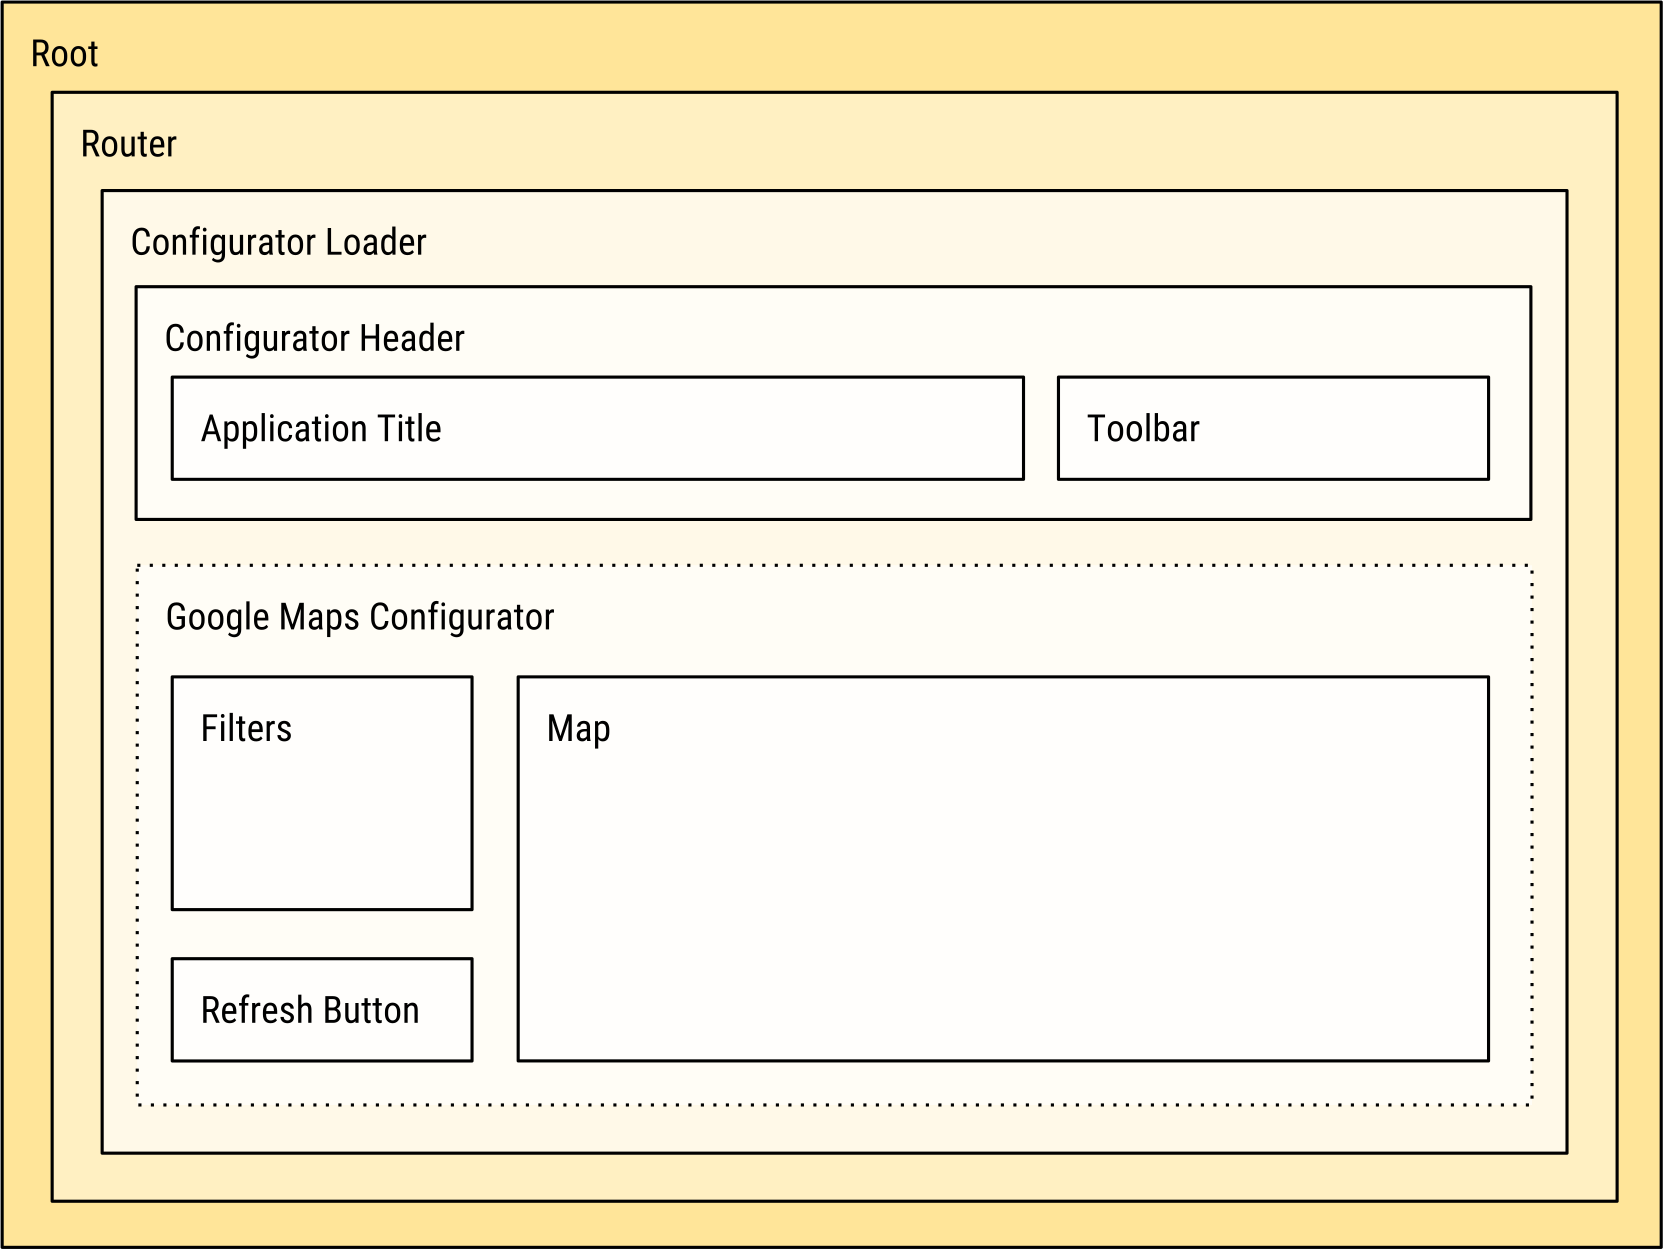
\includegraphics[width=120mm]{img/04_frontend_react_component_hierarchy.png}
	\caption{The hierarchical component representation of a screen containing a \emph{configurator interface}, as suggested on the mockup Figure \ref{fig:mockups_configurator}. The component with the dotted border is the component representing the \emph{configurator interface}. Each \emph{visualizer} defines its own configurator component.} 
	\label{fig:frontend-react-component-hierarchy}
\end{figure}

Let us now talk more in detail about individual parts of this architecture. The actual user interface, i.e. the \emph{controller-view} layer, is composed of hierarchically structured UI components, specifically React~\cite{react} components. On the mockup Figure~\ref{fig:mockups_configurator} we suggested how a screen with a \emph{configurator interface} should look like. Now you can refer to Figure \ref{fig:frontend-react-component-hierarchy} to see how this screen would be represented with the component hierarchy.

An UI component is the base building block that we work with while creating the user interface. It works as a \emph{view}, defining how it should be rendered on the screen, and also as a \emph{controller}, defining how it should respond to user interactions. The main asset of this component approach is composability. One component typically consists of several smaller components, creating as many levels of abstraction as necessary. This can be nicely seen  on Figure \ref{fig:frontend-react-component-hierarchy}. One consequence is that even though we talk about a \emph{controller-view} layer, some components are rather \emph{controllers}, focusing on the application logic, and some are rather \emph{views}, focusing on the visual aspect.
\begin{figure}
	\centering
	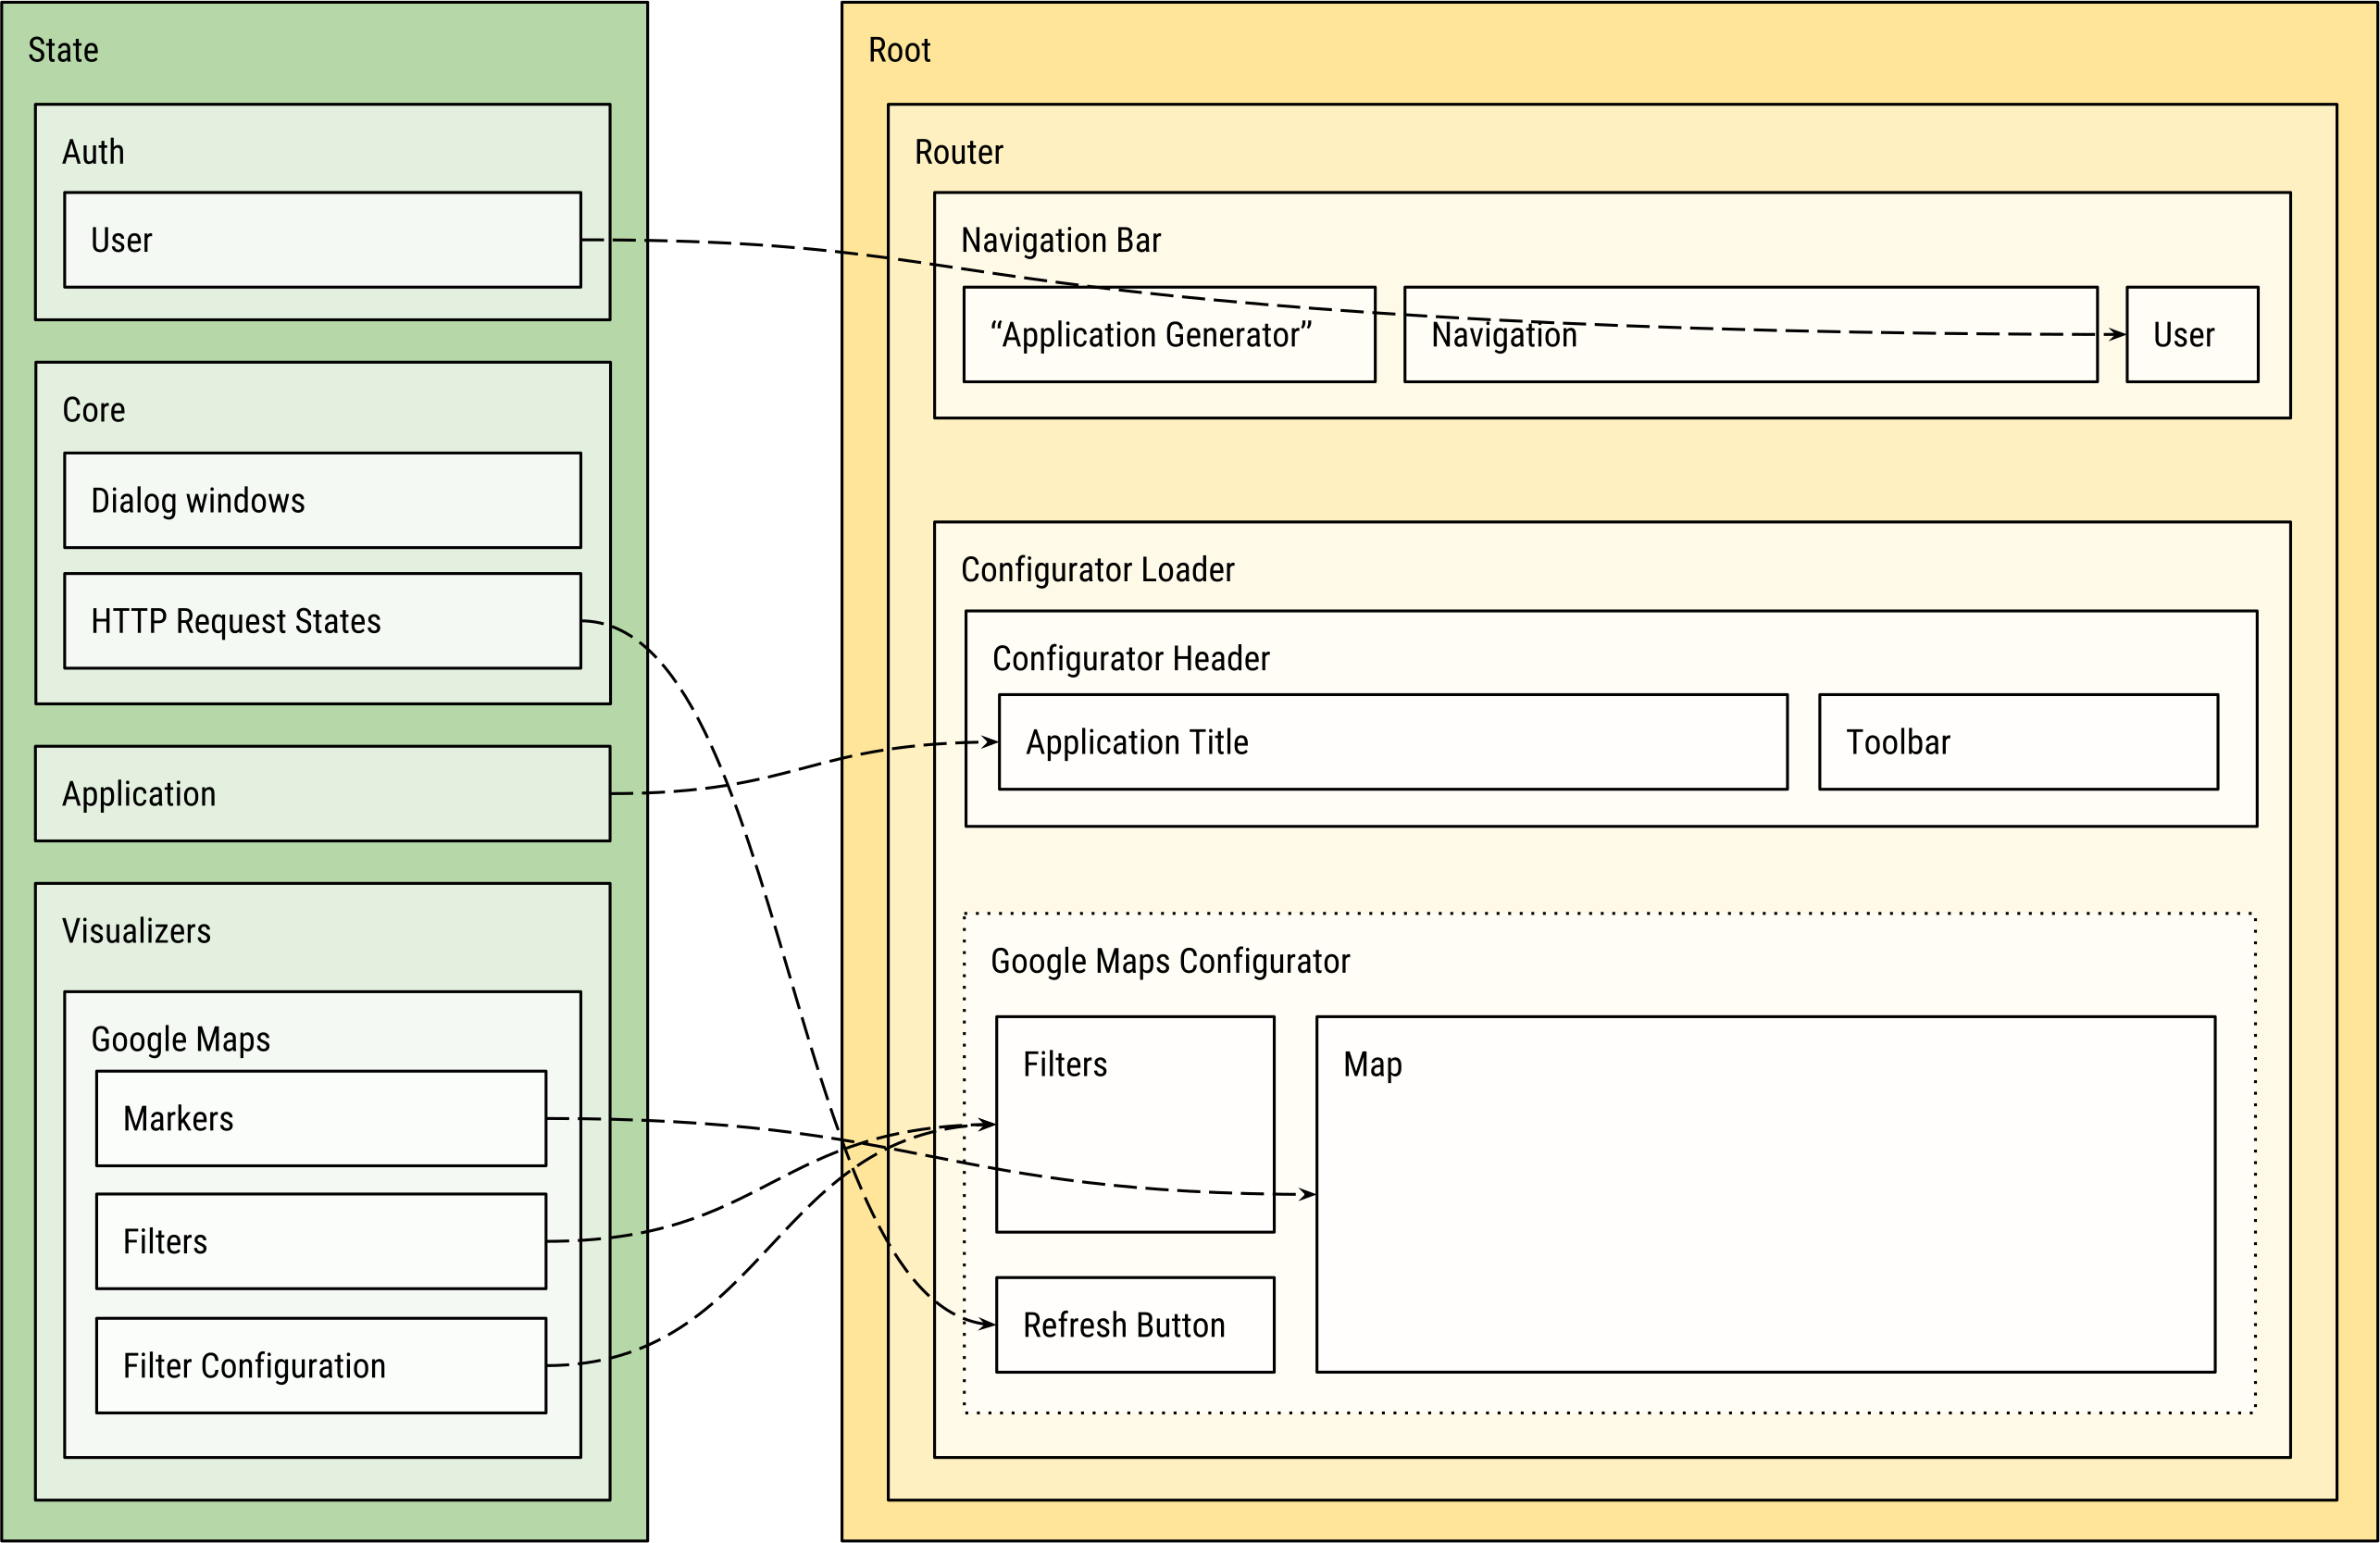
\includegraphics[width=140mm]{img/04_frontend_state_structure.png}
	\caption{The \emph{state} hierarchy mapped to the user interface. Unlike on Figure~\ref{fig:frontend-react-component-hierarchy}, the user interface contains an universal navigation bar that is displayed on top of the screen across the whole platform (among other things it shows the currently authenticated user).} 
	\label{fig:frontend-state-structure}
\end{figure}

The \emph{state} is similarly structured as the user interface, even though the hierarchies are not identical. Figure \ref{fig:frontend-state-structure} gives the reader an idea of what kind of information the \emph{state} actually contains and how this information is mapped to the user interface. 

The role of the \emph{state} is similar to how RDBMS is used in the backend. It works as a structured storage of data (instead of tables we have an arbitrarily deep nested hierarchy). Whereas in backend repositories typically work as the first abstraction layer through which the RDBMS is accessed, in frontend we utilize \emph{reducers} to define how the \emph{state} should be updated using \emph{action}, and \emph{selectors} to select specific data from the \emph{state}. Note that both \emph{reducers} and \emph{selectors} always work only on a single piece of the whole \emph{state}.

Figure \ref{fig:frontend-reducer-and-selector} shows how these concepts are utilized in a real situation. After successful authentication with the backend, the \texttt{SIGN\_IN} action carrying the current user is dispatched. The \texttt{User Reducer} updates the \emph{state} (stores the authenticated user) and the \emph{User Selector} selects the user from the \emph{state} and passes it to a UI component.
\begin{figure}
	\centering
	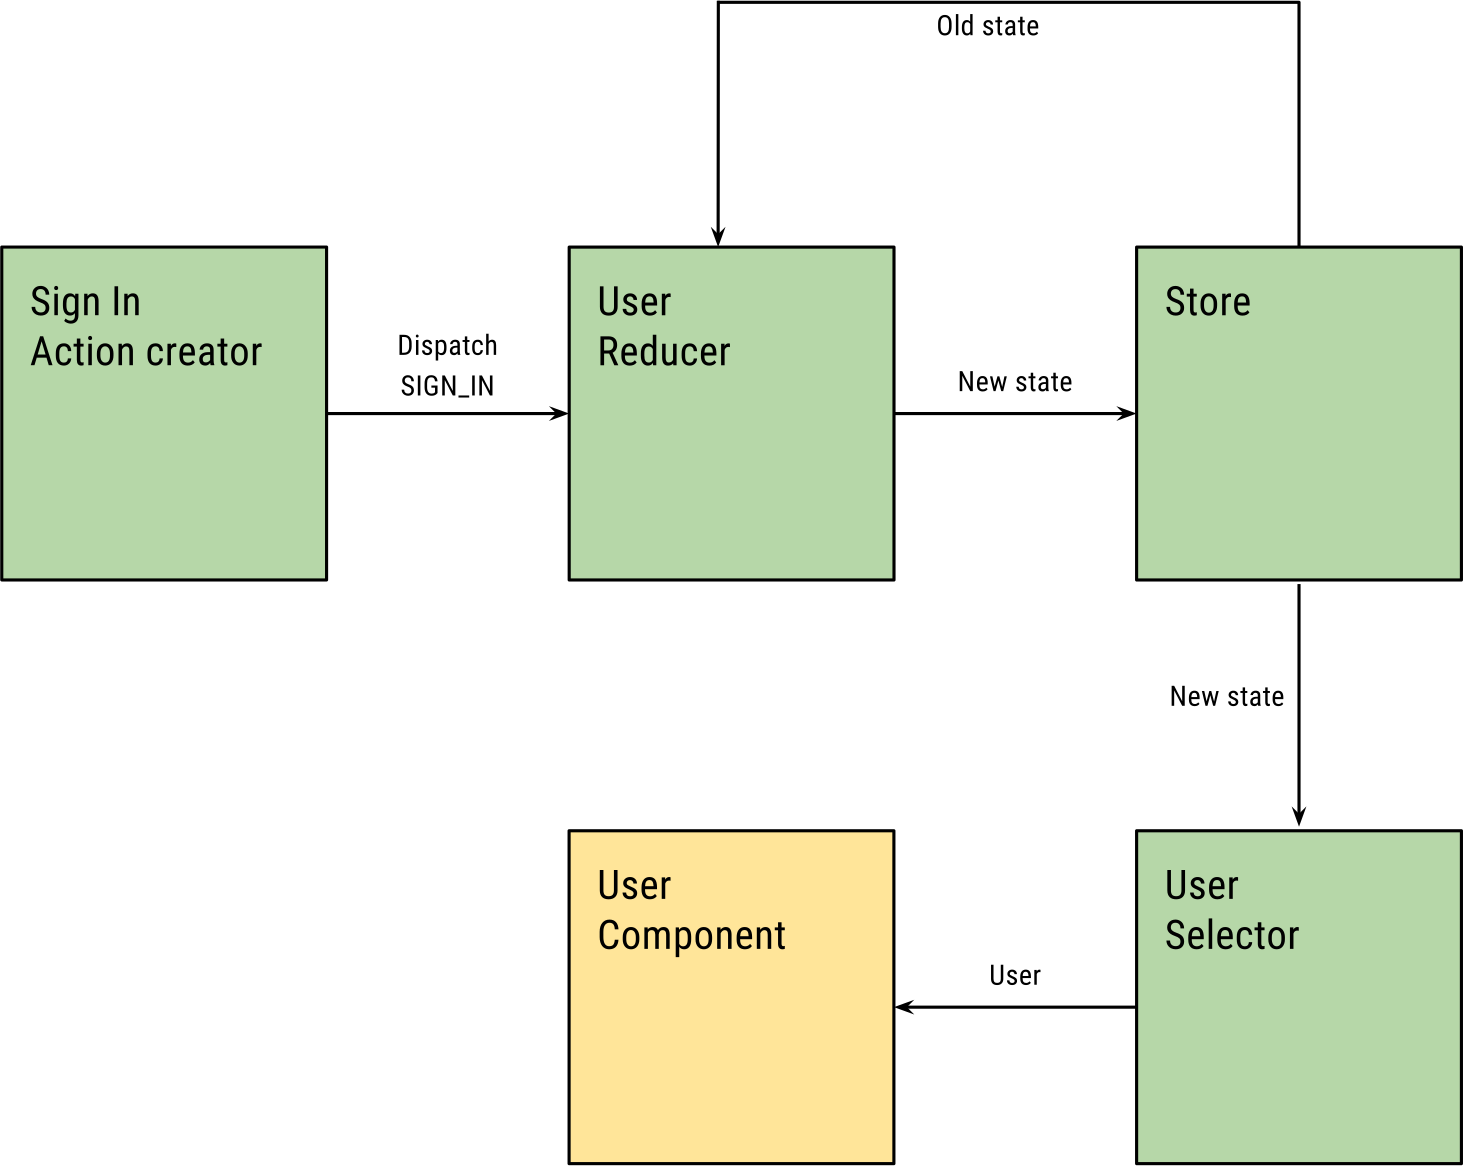
\includegraphics[width=120mm]{img/04_frontend_reducer_and_selector.png}
	\caption{Example showing how a \emph{reducer} is used to update the \emph{state} and how a \emph{selector} is used to obtain a specific piece of information from the \emph{state}.} 
	\label{fig:frontend-reducer-and-selector}
\end{figure}

There is a clear analogy between repositories and the combination of \emph{actions}, \emph{reducers} and \emph{selectors}. \emph{Actions} define API for updates (setters), \emph{selectors} for reads (getters). \emph{Reducers} represent the actual implementations of the setters. \emph{Action creators}, on the other hand,  constitute a higher level of abstraction as they handle more complex tasks from the business logic (such as communication with the backend, as shown in the example on Figure \ref{fig:frontend-making-http-request}). 

Whereas in backend all this functionality is tightly bundled in a single repository or service object (object as in OOP), in backend the individual parts are represented as functions that are coupled only loosely. Nevertheless, we use a name \emph{duck} to refer to a unit of related \emph{actions}, \emph{action creators}, \emph{selectors} and \emph{reducers} that cover a limited functionality (e.g. users). Just as there are different repositories and services in backend, having different responsibilities, there are different \emph{ducks} in frontend. Here are some examples (the \emph{state} structure on Figure~\ref{fig:frontend-state-structure} might have already given some ideas to the user):

\begin{itemize}
\item \textbf{User} -- authenticated user
\item \textbf{Dialog windows} -- state of opened dialog windows
\item \textbf{Promises} -- state of all asynchronous operations in the system (typically HTTP requests to the backend)
\item \textbf{Notifications }-- on-screen user notifications
\item \textbf{Discovery} -- state of the currently opened discovery
\item \textbf{Published applications} -- list of published applications (catalog content)
\end{itemize}

These were just some of the many that exist in the frontend, plus they are typically related to the general \emph{platform} functionality. Then every \emph{visualizer} would define its own \emph{ducks}, typically responsible for fetching and storing the RDF data from the backend and for the \emph{configuration} (as seen on Figure~\ref{fig:frontend-state-structure}).

The last missing piece of the frontend architecture is routing. Despite the frontend being an SPA, standard URLs are still used for identification of different screens, i.e., by changing the current URL the user transitions to another screen. In a typical OOP MVC implementation as is used in the backend, a URL is mapped onto a controller object method. In our frontend application, each URL is mapped on a hierarchy of UI components. 

Let us consider the screen with Google Maps Visualizer \emph{configurator interface} as mocked up on Figure~\ref{fig:mockups_configurator}, with component structure shown on Figure~\ref{fig:frontend-react-component-hierarchy}. Note that this applies only to the \emph{platform} SPA. The URL of this screen is \texttt{/app/13/googleMaps}. The mapping on a component hierarchy would be following:

\begin{itemize}
\item \texttt{app} -- \texttt{Configurator Loader} component
\item \texttt{13} -- the ID of current application. It is passed as a parameter to the \texttt{Configurator Loader} component
\item \texttt{googleMaps} -- \texttt{Google Maps Configurator} component
\end{itemize}

On Figure~\ref{fig:frontend-react-component-hierarchy} there is a \texttt{Router} component high up in the hierarchy. This component is responsible for injecting the components that map on the current URL into the hierarchy. If any segment of the URL changes, the \texttt{Router} replaces the old component with a new one that maps on the new URL segment which results in a screen update. Note the hierarchical nature of this routing approach. 

This suggests how the internal mechanism for loading the appropriate \emph{configurator interface} works. Each \emph{visualizer} defines its own \emph{configurator interface} in a form of a UI component which is seemingly integrated into the component hierarchy (see Figure~\ref{fig:frontend-react-component-hierarchy} where the configurator component is highlighted with a dotted border). Each such component maps on a unique URL. When a user decides to configure an application, he is redirected to this URL and the \emph{Router} activates the appropriate component. 

\subsection{Backend}
\label{sec:system-proposal:architecture-analysis:backend}

The backend of LinkedPipes Visualization is a standard MVC application, consisting of a \emph{Model} layer, containing various repositories and services that handle the business logic, and \emph{Controllers}, defining the public remote API. The integration of our \emph{application generator} into LinkedPipes Visualization is a matter of adding new controllers, repositories and services to the codebase that will cover the new functionality (Figure~\ref{fig:proposed-application-generator-architecture}).

The vast majority of controllers in both LinkedPipes Visualization and the \emph{application generator} handle the asynchronous HTTP requests coming from the frontend. The role of a controller in this typical case is just to translate the HTTP request into an API call to the \emph{Model} layer and send the response back. All controllers together define a public remote API interface.

Even though we could re-use some of the API methods available from the LinkedPipes Visualization controllers (e.g. those for controlling the \emph{discovery} algorithm), we decided not to do that to avoid hidden dependencies between the frontend and the backend. Dependencies within the  codebase (for example between the \emph{Controller} layer and the \emph{Model} layer) are easy to discover using a static program analysis. Simply put, the whole backend is one piece of code and so if there is a broken dependency, the code will not compile. That is not true for the remote API. Therefore the \emph{application generator} frontend strictly uses only those remote API methods that are handled by the \emph{application generator} controllers (as seen on Figure \ref{fig:proposed-application-generator-architecture}). 

The \emph{Model} layer consists of various repositories and services that handle the business logic. Each repository (or a service) covers a limited area of functionality and exposes a clearly defined public API. Whereas repositories usually work on a lower level, providing for example basic access to RDBMS, services involve a higher level logic.

The new services and repositories that are part of the \emph{application generator} are either completely independent (e.g. service handling the users) or create a one-way dependency on some of the existing repositories or services from LinkedPipes Visualization (this can also be seen on Figure \ref{fig:proposed-application-generator-architecture}). For example, there is a \texttt{PipelineDiscoveryRepository} in the original LinkedPipes Visualization codebase that can return a list of executed LDVM \emph{discoveries}. This repository is, however, completely unaware of users. So we implemented our own custom service, \texttt{DiscoveriesService}, that utilizes the aforementioned repository and adds all the extra functionality related to users (e.g. it can return list of executed \emph{discoveries} by a given user).

Figure \ref{fig:proposed-application-generator-architecture} might suggest that our extension of the \emph{Model} layer directly communicates with RDBMS. Strictly speaking, that is not true because we are utilizing some low level services to access the database and those services could still be considered part of the \emph{Model} layer.

\subsection{Separation from LinkedPipes Visualization}

What is important is that all \emph{application generator} related functionality, even though within the same codebase, is kept separated. The frontend communicates only with our controllers. The backend extension is in a form of a compact layer over the original codebase, consisting of custom controllers, services and repositories. The dependencies on the original codebase, as shown on Figure~\ref{fig:proposed-application-generator-architecture}, are always in a form of utilizing the internal API of LinkedPipes Visualization. It is easy to draw the line where LinkedPipes Visualization ends and our \emph{application generator} begins. Only in rare cases, we re-use some low-level utilities from the original codebase.

\subsection{Extendability with new visualizers}
\label{sec:system-proposal:architecture-analysis:extendability}

Let us now talk about one distinct feature that the software architecture needs to count with: extendability. In this case, it specifically means the ability to be extended with new \emph{visualizers}. As we have described, a \emph{visualizer} (Subsection \ref{sec:linkedpipes:visualizers}) consists of an RDF definition of the LDVM \emph{component} and a \emph{plugin}. The RDF definition needs to be simply imported to the LDVM instance so that the \emph{discovery} algorithm can start using it. The situation is more complicated with the \emph{plugin} as it needs to be properly integrated both in the backend and in the frontend. How this is done can be seen on Figure \ref{fig:sample-visualizer-structure}.

\begin{figure}
	\centering
	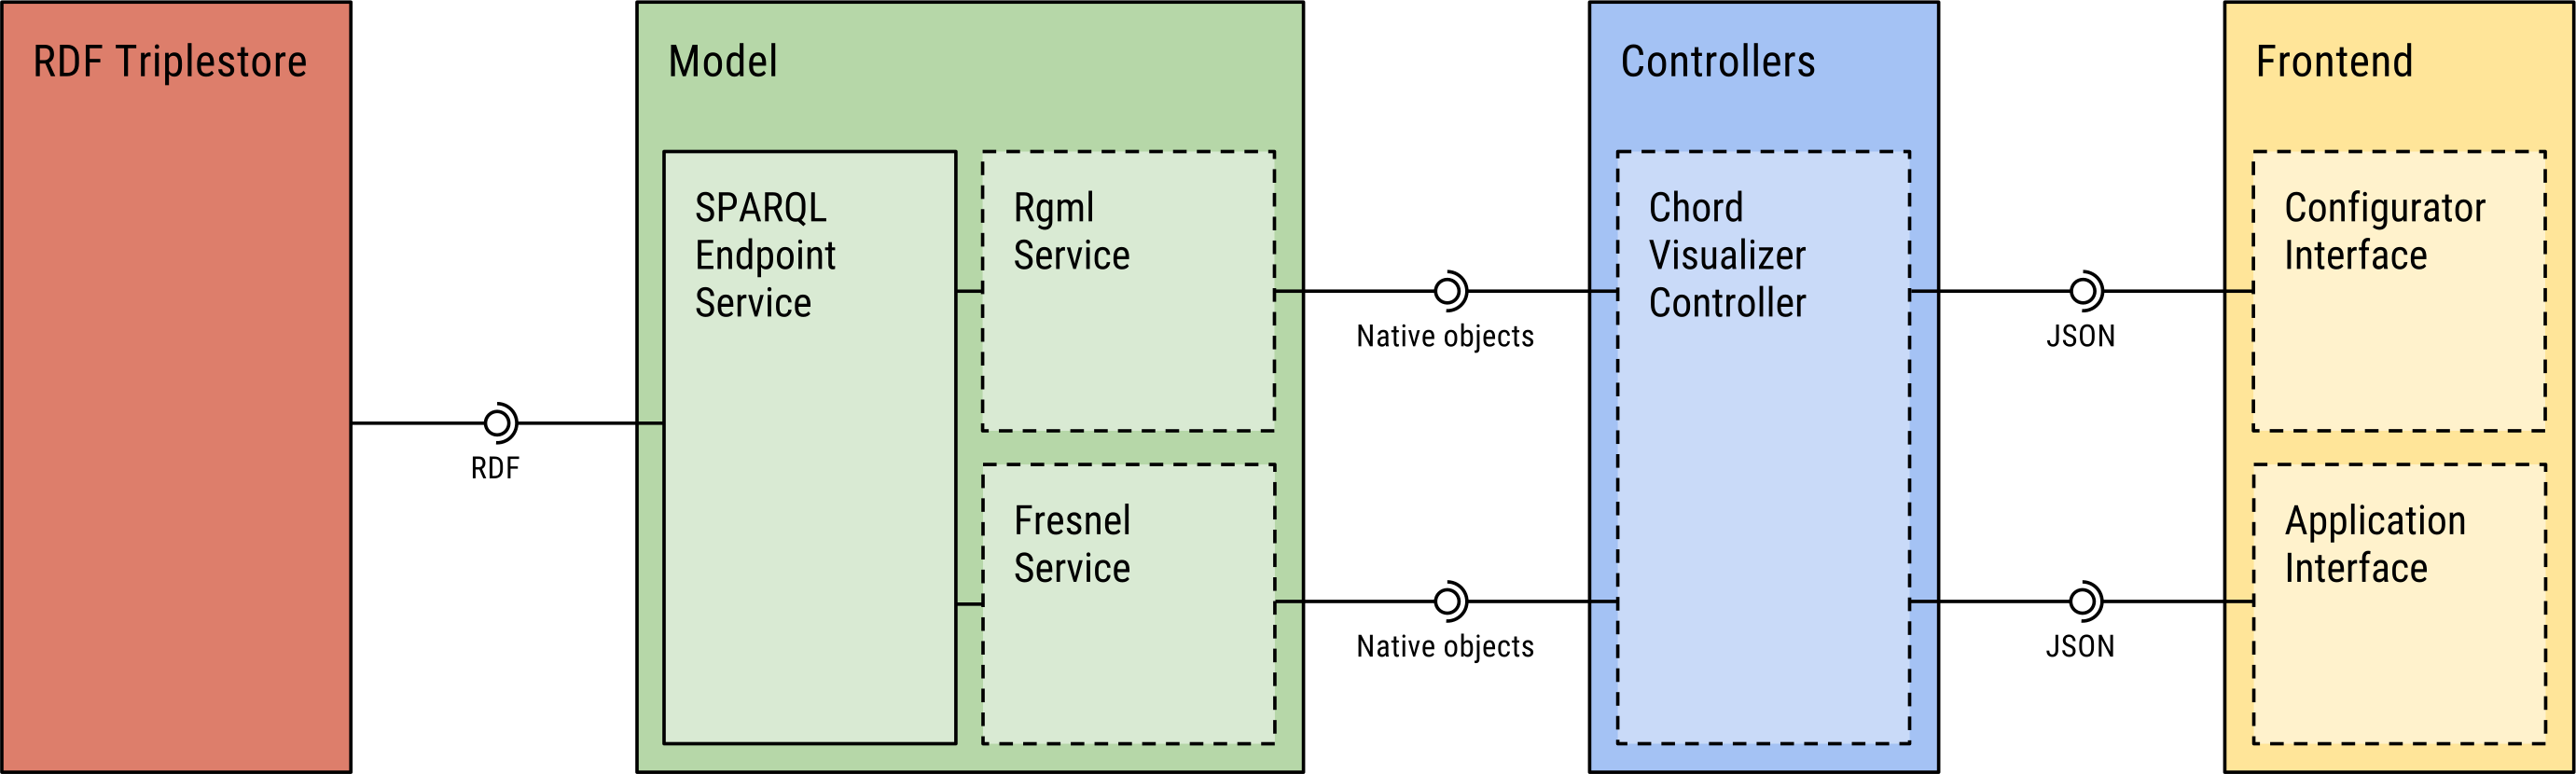
\includegraphics[width=140mm]{img/04_chord_visualizer_structure.png}
	\caption{Architecture of a sample \emph{visualizer}, D3.js Chord Visualizer, showing how it is integrated into the \emph{application generator}. The blocks with dashed borders represent newly implemented components. The label underneath each connections suggests the data format of that particular API.} 
	\label{fig:sample-visualizer-structure}
\end{figure}

The backend part is typically responsible for converting the data from RDF to a format suitable for the visualizer frontend. This functionality is exposed via a remote API that the frontend can utilize. What is important is that individual API methods are rather independent. As long as we keep some kind of system in the API method URLs to avoid conflicts (e.g. define a unique URL prefix for each \emph{visualizer}), we can almost indefinitely extend the API with new methods by adding new controllers and extending the old ones. Obviously, the actual business logic is handled in the \emph{Model} layer but that can be extended in similar manner with new repositories and services.

As we are specifically talking about the backed part of a new \emph{visualizer}, this extension would typically involve a new service adding support for a new RDF vocabulary.  Such a service would have a fairly simple structure as it would most likely just expose methods that take input RDF data as an argument and return the data represented in native domain objects (that will be eventually converted to JSON and sent to the frontend). Given this structure, we can easily add as many similar services to support as many vocabularies as we need without worrying about any conflicts. The extendability is rather straightforward.

On the other hand, each such service would heavily depend on the internal RDF infrastructure of LinkedPipes Visualization. This infrastructure not only provides among other things services to access the triplestore but also defines various conventions for example for how a SPARQL should be expressed in the native code. This is the only case when our code significantly overlaps with the original LinkedPipes Visualization code.

The frontend part contains the \emph{configurator} and \emph{application} interfaces. They both need to be integrated into the rest of the frontend which is a rather complex task. Firstly, there must be a mechanism that based on the application type (i.e., the LDVM \emph{visualizer} component) dynamically selects the correct \emph{configurator} (or \emph{application}) interface and shows it to the user. Secondly, not only does the (let us say) \emph{configurator} interface have to be able to communicate with the rest of the frontend, but it also should  look like it is a part of it, i.e., it should fit in and follow the recommended visual design guidelines. 

We partially described this process in Section~\ref{sec:system-proposal:architecture-analysis:frontend-architecture}. The frontend user interface is defined using a hierarchy of \emph{controller-view} components. Both the \emph{configurator} and \emph{application} interfaces are in a form of such a component that is seemingly integrated into the component hierarchy. The mechanism that dynamically selects an appropriate component depending on a \emph{visualizer} has been also described in Section~\ref{sec:system-proposal:architecture-analysis:frontend-architecture}. 

We have also mentioned a concept of \emph{ducks} which corresponds to the concept of repositories and services in backend. Therefore extending the frontend with a new \emph{visualizer} does not only involve implementing UI components for the \emph{configurator}  and \emph{application} interfaces, but also usually means adding new \emph{ducks} that handle the frontend business logic of this \emph{visualizer}. This functionality typically involve utilizing the backend \emph{visualizer} API (e.g. loading the data to be visualized) and also the \emph{visualizer} configuration.

\subsection{Steps to implement a new visualizer}

Let us summarize the previous subsection by simply listing the base tasks necessary to integrate a new \emph{visualizer} to the \emph{application generator}. Note that the tasks are not numbered. Clearly, one has to start with defining the RDF data format (i.e., how the input data for the \emph{visualizer} should look like) and with designing the API. Once this is done, the order in which the following tasks are carried out is irrelevant.

\begin{itemize}
\item Define and add the LDVM \emph{visualizer} component so that the \emph{discovery} algorithm can use it.
\item Implement necessary services in the \emph{Model} layer that extract RDF data in custom vocabularies and convert them to native objects.
\item Implement the \emph{visualizer} controller that utilizes the services and exposes their functionality via a public remote API.
\item Implement necessary \emph{ducks} that cover the \emph{visualizer} frontend functionality (specifically loading the data to be visualized).
\item Implement the \emph{configurator} and \emph{application} components and integrate them into the frontend. 
\end{itemize}

\subsection{API design}

The whole application consists of separate layers (Figure \ref{fig:proposed-application-generator-architecture}). On the top level the application is split into the frontend and the backend. The backend is then organized into layers as well, according to the MVC architecture. Finally, the \emph{Model} layer typically consists of multiple levels of abstraction for each problem it covers (repositories, services etc). Each layer defines a public API using which it can be utilized by higher layers.

Let us talk for now about the public remote HTTP API that is exposed by the backend, i.e., the API that is used for the communication between the frontend and the backend. The API consists of many smaller APIs that each covers a limited area of functionality and is represented by a single controller. All the controllers together cover everything that is required by the frontend, i.e., the complete functionality of the \emph{application generator} (remember that on this level, we are not utilizing anything from the original API of LinkedPipes Visualization at all). Let us now walk through the base individual APIs which will give the reader an idea of what the \emph{application generator} do and how it works.

\begin{itemize}
\item \textbf{Application API} -- returns a generated application and its configuration.
\item \textbf{Authentication API} -- authentication and registration of users.
\item \textbf{Catalog API} -- browsing through the catalog of published applications.
\item \textbf{Common Visualizer API} -- common functionality for all visualizers (e.g. dereferencing labels).
\item \textbf{Create Application API} -- the process of creating an application which includes browsing data sources, running the \emph{discovery}, executing selected \emph{pipelines}.
\item \textbf{Dashboard API} -- browsing and basic management of the user content, which includes applications, data sources and \emph{discoveries}.
\item \textbf{Manage Application API} -- updating, deleting and configuring a generated application.
\end{itemize}

These APIs cover the general agenda of the \emph{application generator}. Then each \emph{visualizer} defines its own API (its own controller, see Figure \ref{fig:sample-visualizer-structure}) that covers only the functionality of this particular \emph{visualizer} (note that this is rather a convention). Also note that some of the APIs are completely public (e.g the \textbf{Catalog API}), most of them, however, require the user to be authenticated.

Let us now  have a look at a short scenario showing how the API works. In this scenario, the user will initiate the LDVM \emph{discovery} algorithm and then watch the progress on the screen.

In the preceding step, the user selected the data sources he is interested in. Now he clicks the "Run Discovery" button to initialize the \emph{discovery}. The whole process can be seen on Figure \ref{fig:api-run-discovery-diagram}. The frontend makes an asynchronous HTTP request to the backend. The request is first processed on the \emph{Controller} layer which, among other things, verifies that the user is properly authenticated. The request is then passed on to the \emph{Model} layer where the \texttt{Pipeline Service} starts the actual \emph{discovery} of selected data sources. The \emph{discovery} might take some time so the request does not wait for it to finish. The \texttt{Pipeline Service} simply returns an ID assigned to this particular \emph{discovery}. This ID is what is finally delivered back to the frontend.

\begin{figure}
	\centering
	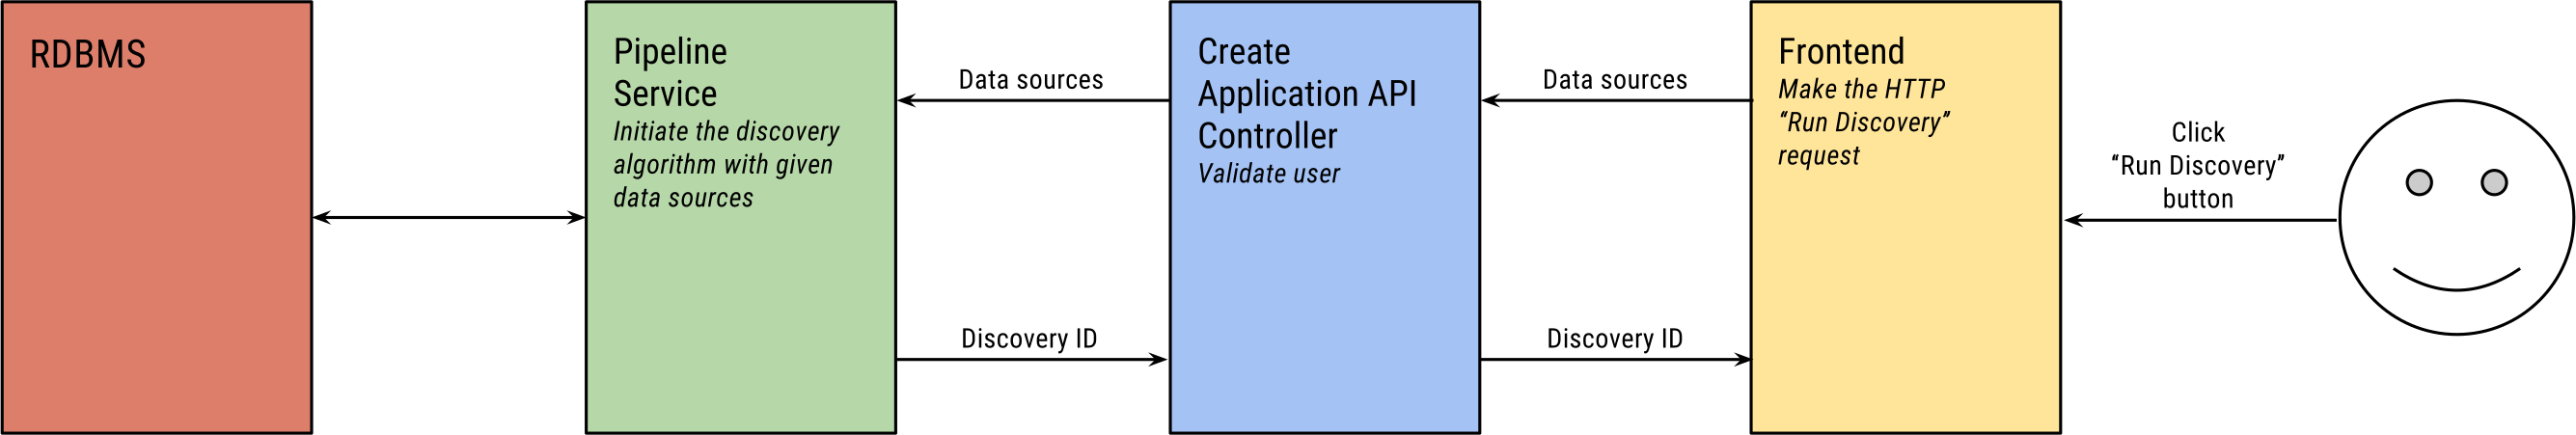
\includegraphics[width=140mm]{img/04_api_run_discovery_diagram.png}
	\caption{Diagram showing the process of running the \emph{discovery} algorithm from the API perspective. The face represents the user initiating the request.} 
	\label{fig:api-run-discovery-diagram}
\end{figure}

As the \emph{discovery} continues, it updates its current status in RDBMS. It also stores to RDBMS the \emph{pipelines} that has been discovered so far. The frontend uses the acquired \emph{discovery} ID to periodically poll the backend for this information until the \emph{discovery} finishes. This way the user can see online on the screen the current status of the \emph{discovery} and also the discovered \emph{pipelines}. This request can be seen on Figure \ref{fig:api-get-discovery-diagram}.

In LinkedPipes Visualization, this particular part is implemented differently. Instead of periodical polling, the \emph{discovery} algorithm output flows through a WebSocket \footnote{\url{https://tools.ietf.org/html/rfc6455}} which is opened between the frontend and the backend. In many ways this solution is more elegant. Only one connection has to be maintained and the updates are pushed to the frontend almost instantly. Unfortunately, in the current implementation in LinkedPipes Visualization, once a WebSocket to a particular \emph{discovery} is closed (e.g. because the user closes the page), it cannot be re-opened again. That means that the user loses the option to watch the \emph{discovery} algorithm progress online. In this sense, our implementation is better as it allows the user to leave and come back anytime later. If the \emph{discovery} has not finished yet, the polling is automatically restored.
\begin{figure}
	\centering
	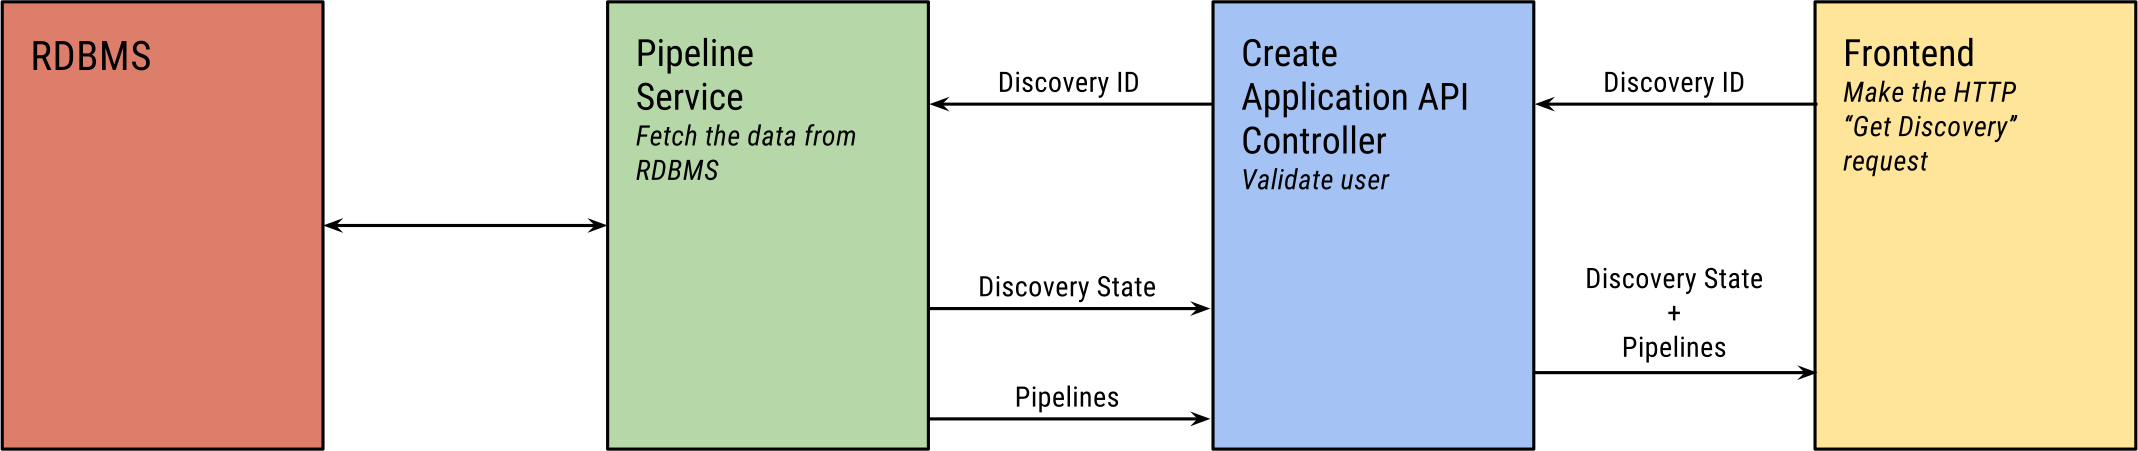
\includegraphics[width=140mm]{img/04_api_get_discovery_diagram.png}
	\caption{Diagram showing the process of fetching the \emph{discovery} algorithm status and the discovered pipelines from the API perspective.} 
	\label{fig:api-get-discovery-diagram}
\end{figure}





